%% (Master) Thesis template
% Template version used: v1.4
%
% Largely adapted from Adrian Nievergelt's template for the ADPS
% (lecture notes) project.

%% We use the memoir class because it offers a many easy to use features.
\documentclass[11pt,a4paper,titlepage]{memoir}

%\usepackage[a4paper, left=1in, right=1in, bottom=1in, top=0.75in]{geometry}
 
%% Packages
%% ========

%% Some more packages that you may want to use.  Have a look at the
%% file, and consult the package docs for each.
%% See the TeXed file for more explanations

%% LaTeX Font encoding -- DO NOT CHANGE
\usepackage[OT1]{fontenc}

%% Babel provides support for languages.  'english' uses British
%% English hyphenation and text snippets like "Figure" and
%% "Theorem". Use the option 'ngerman' if your document is in German.
%% Use 'american' for American English.  Note that if you change this,
%% the next LaTeX run may show spurious errors.  Simply run it again.
%% If they persist, remove the .aux file and try again.
\usepackage[english]{babel}

%% Input encoding 'utf8'. In some cases you might need 'utf8x' for
%% extra symbols. Not all editors, especially on Windows, are UTF-8
%% capable, so you may want to use 'latin1' instead.
\usepackage[utf8]{inputenc}

%% This changes default fonts for both text and math mode to use Herman Zapfs
%% excellent Palatino font.  Do not change this.
%\usepackage[sc]{mathpazo}
\usepackage{lmodern}
%\usepackage[italic]{mathastext}
%\usepackage{newpxtext, newpxmath}
%\usepackage{newtx}

%% The AMS-LaTeX extensions for mathematical typesetting.  Do not
%% remove.
\usepackage{amsmath, bm, amssymb} %,,amsfonts,mathrsfs,

%% NTheorem is a reimplementation of the AMS Theorem package. This
%% will allow us to typeset theorems like examples, proofs and
%% similar.  Do not remove.
%% NOTE: Must be loaded AFTER amsmath, or the \qed placement will
%% break
\usepackage[amsmath,thmmarks]{ntheorem}

%% Newcommands
%\newtheorem*{definition*}{\textit{Definition.}}
%\newtheorem*{proof*}{\textit{Proof.}}
%\newtheorem{definition}{Definition}
\newcommand*{\code}{\lstinline[keepspaces=true,breaklines]}
\newcommand\x{0.28}

%% LaTeX' own graphics handling
\usepackage{graphicx}
\graphicspath{ {./images/} }
\usepackage{wrapfig}

%% Draw maps
\usepackage{tikz}
\usetikzlibrary{shapes.geometric}

%% Tables
\usepackage{capt-of}% or \usepackage{caption}
\usepackage{booktabs}
\usepackage{varwidth}

%% Valign
\usepackage[export]{adjustbox} % for valign option

%% We unfortunately need this for the Rules chapter.  Remove it
%% afterwards; or at least NEVER use its underlining features.
% \usepackage{soul}

%% declaration of originality.
\usepackage{pdfpages}

%% [NEED] This allows for additional typesetting tools in mathmode.
%% See its excellent documentation.
\usepackage{mathtools}

%% [NEED] Some extensions to tabulars and array environments.
\usepackage{array}

%% [OPT] Fancy package for source code listings.  The template text
%% needs it for some LaTeX snippets; remove/adapt the \lstset when you
%% remove the template content.
\usepackage{listings}
\lstset{language=TeX,basicstyle={\normalfont\ttfamily}}

%% [REC] Fancy character protrusion.  Must be loaded after all fonts.
%\usepackage[activate]{pdfcprot}

%% Make document internal hyperlinks wherever possible. (TOC, references)
%% This MUST be loaded after varioref, which is loaded in 'extrapackages'
%% above.  We just load it last to be safe.
\usepackage{hyperref} 
\hypersetup{colorlinks=true,
            linkcolor=blue,
            anchorcolor=black,
            citecolor=green,
            filecolor=cyan,
            menucolor=red,
            runcolor=cyan,
            urlcolor=cyan}

\usepackage[backref=true, backend=biber, style=phys]{biblatex} %Imports biblatex package
\emergencystretch=1em
\setcounter{biburllcpenalty}{7000}
\setcounter{biburlucpenalty}{8000}

\DefineBibliographyStrings{english}{%
  backrefpage = {page},% originally "cited on page"
  backrefpages = {pages},% originally "cited on pages"
}

\addbibresource{refs.bib} %Import the bibliography file
\usepackage{csquotes} % compatibility with biblatex

\usepackage{enumitem}
\setlist[itemize]{leftmargin=*}
%% Our layout configuration.  DO NOT CHANGE.
%% Memoir layout setup

%% NOTE: You are strongly advised not to change any of them unless you
%% know what you are doing.  These settings strongly interact in the
%% final look of the document.

% Dependencies
\usepackage{ETHlogo}

% Turn extra space before chapter headings off.
\setlength{\beforechapskip}{0pt}

\nonzeroparskip
\parindent=0pt
\defaultlists

% Chapter style redefinition
\makeatletter

\if@twoside
  \pagestyle{Ruled}
  \copypagestyle{chapter}{Ruled}
\else
  \pagestyle{ruled}
  \copypagestyle{chapter}{ruled}
\fi
\makeoddhead{chapter}{}{}{}
\makeevenhead{chapter}{}{}{}
\makeheadrule{chapter}{\textwidth}{0pt}
\copypagestyle{abstract}{empty}

\makechapterstyle{bianchimod}{%
  \chapterstyle{default}
  \renewcommand*{\chapnamefont}{\normalfont\Large\sffamily}
  \renewcommand*{\chapnumfont}{\normalfont\Large\sffamily}
  \renewcommand*{\printchaptername}{%
    \chapnamefont\centering\@chapapp}
  \renewcommand*{\printchapternum}{\chapnumfont {\thechapter}}
  \renewcommand*{\chaptitlefont}{\normalfont\huge\sffamily}
  \renewcommand*{\printchaptertitle}[1]{%
    \hrule\vskip\onelineskip \centering \chaptitlefont\textbf{\vphantom{gyM}##1}\par}
  \renewcommand*{\afterchaptertitle}{\vskip\onelineskip \hrule\vskip
    \afterchapskip}
  \renewcommand*{\printchapternonum}{%
    \vphantom{\chapnumfont {9}}\afterchapternum}}

% Use the newly defined style
\chapterstyle{bianchimod}

\setsecheadstyle{\Large\bfseries\sffamily}
\setsubsecheadstyle{\large\bfseries\sffamily}
\setsubsubsecheadstyle{\bfseries\sffamily}
\setparaheadstyle{\normalsize\bfseries\sffamily}
\setsubparaheadstyle{\normalsize\itshape\sffamily}
\setsubparaindent{0pt}

% Set captions to a more separated style for clearness
\captionnamefont{\sffamily\bfseries\footnotesize}
\captiontitlefont{\sffamily\footnotesize}
\setlength{\intextsep}{16pt}
\setlength{\belowcaptionskip}{1pt}

% Set section and TOC numbering depth to subsection
\setsecnumdepth{subsection}
\settocdepth{subsection}

%% Titlepage adjustments

\pretitle{\par\vspace{0pt plus 0.7fill}\centering\HUGE\sffamily\bfseries}\posttitle{\par}
\preauthor{\centering\let\and\\\Large\sffamily}\postauthor{\par}
\predate{\centering\par\Large\sffamily}\postdate{\par}


\def\@advisors{}
\newcommand{\advisors}[1]{\def\@advisors{#1}}
\def\@department{}
\newcommand{\department}[1]{\def\@department{#1}}
\def\@thesistype{}
\newcommand{\thesistype}[1]{\def\@thesistype{#1}}

\renewcommand{\maketitlehooka}{\noindent\ETHlogo[2in]}

\renewcommand{\maketitlehookb}{\vspace{1in}%
  \par\begin{center}\Large\sffamily\@thesistype\end{center}}

\renewcommand{\maketitlehookd}{%
  \vfill\par
  \begin{flushright}
    \sffamily
    \@advisors\par
    \@department, ETH Z\"urich
  \end{flushright}
}

\checkandfixthelayout

\setlength{\droptitle}{-48pt}

\makeatother

% This defines how theorems should look. Best leave as is.
%\theoremstyle{plain}
%\setlength\theorempostskipamount{0pt}

%%% Local Variables:
%%% mode: latex
%%% TeX-master: "thesis"
%%% End:


%% Document information
%% ====================

\title{Weak lensing map inference: a physics informed Gaussian process approach}
%\title{Weak lensing map inference with physics informed Gaussian process}
\author{Nicolò Massari}
\thesistype{Master Thesis}
\advisors{Advisors: 
                    Prof.\ Dr.\ Alexandre Réfrégier,
                    Dr.\ Tilman Tröster.
                    Veronika Oehl}
\department{Department of Physics}
\date{April 02, 2024}

\begin{document}

\frontmatter

%% Title page is autogenerated from document information above.  DO
%% NOT CHANGE.
\begin{titlingpage}
\calccentering{\unitlength}
\begin{adjustwidth*}{\unitlength-24pt}{-\unitlength-24pt}
\maketitle
\end{adjustwidth*}
\end{titlingpage}

%% The abstract of your thesis.  Edit the file as needed.
%%%%%%%%%%%%%%%%%%%%%%%%%%%%%%%%%
%%%%%%%%%%%% CHAPTER %%%%%%%%%%%%
%%%%%%%%%%%%%%%%%%%%%%%%%%%%%%%%%
\begin{abstract}
In this work we propose the use of physically informed Gaussian processes (GP) to analyse cosmological fields at the map level. We will show that GPs can capture the statistical behaviour of cosmological fields, providing us with a likelihood as a function of the cosmological parameters conditioned to the map. In practice, we set the Gaussian process kernel to be the 2-point autocorrelation function associated to a 2D discrete flat-sky convergence map. We find that a GP in this setup is not only able to generate maps with the wanted 2-point statistics, but also to reconstruct masked data with an associated uncertainty. Additionally, we perform a Bayesian inference analysis in order to test the ability of Gaussian processes to recover cosmological parameters. We find that we are able to consistently recover the $\sigma_8$ and $\Omega_m$ degeneracy, recovering $S_8$ within two sigma uncertainty. The data is simulated by a Gaussian random field realisation of a convergence map of size $(10^{\circ},10^{\circ})$, $64\times64$ grid, mask $\sim 10\%$ and noise given by a galaxy density of $n_g=10\text{ galaxies}/\text{arcmin}^2$. 

\bigskip

\textit{keywords}: Gaussian processes, weak lensing.
\end{abstract}

%% TOC with the proper setup, do not change.
\cleartorecto
\tableofcontents
\mainmatter

%%%%%%%%%%%%%%%%%%%%%%%%%%%%%%%%%
%%%%%%%%%%%% CHAPTER %%%%%%%%%%%%
%%%%%%%%%%%%%%%%%%%%%%%%%%%%%%%%%
\chapter{Introduction}

Matter bends light. The theory of general relativity predicts that the presence of matter or energy changes the geometry of space and time, which in turn can cause what would otherwise be the straight path of a beam of light to curve. Take a distant source of light. If we assume the universe not to be empty, then between us and said source there exists a non trivial matter disposition. As light travels through everything that is in between us and the source, it gets blocked, bent and distorted. We call this phenomenon weak lensing. In practice what we measure is the shape of distant galaxies. These images do not show a distinct lensing feature individually, as such tiny changes can only be seen with a large number of sources. For example, we observe that galaxies have a tendency of aligning along a preferred axis, causing a statistical discrepancy in an otherwise seemingly isotropic universe. For further details on lensing, please refer to \cite{cosmology:lensing} \cite{cosmology:lensing2}; for weak lensing \cite{weaklensing}. The image of a distant galaxy can change shape or size. Changes in shape are fully characterised by the shear distortion $\Vec{\gamma}$ vector field, where the change in size is given by its magnitude, the convergence field $\kappa$. We lay out a theoretical framework for weak lensing in \textit{Sec. }\ref{sec:weak lensing} as well as details on the cosmology used in this thesis in \textit{Sec. }\ref{subsec:cosmology}.

A lot of work goes into translating a measurement of distant galaxies to its mathematically friendly counterpart $\Vec{\gamma}$. This is one of the reasons why we will not be dealing with it in this thesis, as it is outside of our scope. Instead we will be simulating our own convergence fields. We use a \textit{Gaussian random field (GRF)} algorithm for the creation of Gaussianly distributed data. As well as lognormal transformations to create fields with a distribution that resembles more closely that in our universe. These transformations are listed in \textit{Sec. }\ref{sec:field generation}; we then use them to simulate our data as explained in \textit{Sec. }\ref{sec:data simulation}. We also verify that the generated fields recover the fiducial power spectrum in \textit{Sec. }\ref{sec:gaussian and lognormal fields}.


\begin{wrapfigure}{r}{0.45\textwidth}
\centering
\begin{tikzpicture}
  % Nodes
  \node[diamond, draw=black, fill=black, text=white, minimum size=2.5cm, rounded corners] (a) at (0,0) {$\bm{\Theta}$};
  \node[diamond, draw=black, fill=white, text=black, minimum size=2.5cm, rounded corners] (b) at (0,-3) {$C(\Theta)$};
  \node[diamond, draw=black, fill=white, text=black, minimum size=2.5cm, rounded corners] (c) at (0,-6) {$w(\Theta)$};
  \node[diamond, draw=black, fill=white, text=black, minimum size=2.5cm, rounded corners] (d) at (0,-9) {$\mathcal{GP}(\Theta)$};
  \node[diamond, draw=black, fill=white, text=black, minimum size=2.5cm, rounded corners] (e) at (-3,-12) {$y$};
  \node[diamond, draw=black, fill=black, text=white, minimum size=2.5cm, rounded corners] (f) at (0,-12) {$\bm{\mathcal{L}(\Theta \mid y)}$};

  % Arrows
  \draw[->, line width=1.5pt] (a) -- (b);
  \draw[->, line width=1.5pt] (b) -- (c);
  \draw[->, line width=1.5pt] (c) -- (d);
  \draw[->, line width=1.5pt] (d) -- (f);
  \draw[->, line width=1.5pt] (e) -- (f);

\end{tikzpicture}
\caption{Simplified steps taken by the model to go from cosmological parameters $\Theta$ to likelihood $\mathcal{L}$ using GP. Here $C$ and $w$ stand for the power spectrum and correlation function respectively, $y$ is the data.}
\label{tik:GP pipeline}
\end{wrapfigure}
A \textit{Gaussian process (GP)} usually assumes little prior knowledge about the data it is applied to. Current research in the field of cosmology views GPs as a machine learning tool to be trained. It is used to accelerate and optimise models \cite{gp:acceleration} \cite{gp:acceleration2} \cite{gp:acceleration3}, as well as for its interpolation qualities applied to the reconstruction of functions determining the evolution of the universe \cite{gp:expansion} \cite{gp:expansion2} \cite{gp:expansion3}. Our work, however, is based on a different approach. We apply our prior knowledge about 2-point statistics in cosmology to create a fully informed GP. Restricting ourselves to 2D flat-sky weak lensing convergence fields, as shown in \textit{Fig. }\ref{tik:GP pipeline}, we can:
\begin{itemize}
    \item compute the angular power spectrum $C(\Theta)$ from a set of cosmological parameters $\Theta$,
    \item transform it in the convergence angular autocorrelation function $w(\Theta)$,
    \item create a zero mean GP with kernel given by said correlation function,
    \item evaluate the likelihood $\mathcal{L}$ of $\Theta$ given a set of data points $y$.
\end{itemize}
With a Bayesian approach we make use of this pipeline to infer the values of the cosmological parameters. Running a \textit{Markov chain Monte Carlo (MCMC)} we can sample the posterior distribution of the cosmological parameters, in particular we will get contours for $\Omega_m$, $\sigma_8$ and $S_8$. Other than that, GPs have several other interesting properties at the field level. They are not only able to generate fields that recover the fiducial 2-point statistics, but are also able to reconstruct masked fields, a task that usually brings many challenges to $C_\ell$ estimation \cite{cellestim} \cite{cellestim2}. In the field of weak lensing in particular, foreground objects like bright stars or galaxies can contaminate measurements, leading to the need of masking such a region, essentially removing the signal.

Here we list the advantages of our method:
\begin{itemize}
    \item minimal information loss, as it is a map based method we use all available data points,
    \item it can be used as a likelihood for cosmological parameters inference,
    \item easily deals with masked fields, providing estimates with an associated uncertainty for the masked points.
\end{itemize}
Whilst some of the disadvantages:
\begin{itemize}
    \item the conditioning process depends on the inverse of a correlation matrix, with a computational effort that grows as $\sim \mathcal{O}(n^3)$ for $n\propto$ data points, indicating possible scaling issues;
    \item due to the intrinsic Gaussianity of GPs, the distribution of the samples will be Gaussian, making it hard to apply them to other fields, say for example lognormal fields.
\end{itemize}
GPs in this thesis are presented in a general introduction in \textit{Sec. }\ref{sec:gaussian process}, followed by a detailed account of the computational methods used to recover a working kernel for GPs in \textit{Sec. }\ref{sec:gaussian process kernel}. In our results we show their ability to create maps that follow the desired statistic \textit{Sec. }\ref{sec:gaussian process priors} and reconstruct data \textit{Sec. }\ref{sec:gaussian process map reconstruction}. We also present our attempt at cosmological parameters inference with GPs in \textit{Sec. }\ref{sec:inference of cosmological parameters}.

It is important to note that throughout the thesis we follow the extremely useful guidelines set by the \code{Miko} pipeline \cite{fwdmodel} on how to deal with discrete maps in weak lensing. 

%\cite{cmbmodel?}
%%%%%%%%%%%%%%%%%%%%%%%%%%%%%%%%%
%%%%%%%%%%%% CHAPTER %%%%%%%%%%%%
%%%%%%%%%%%%%%%%%%%%%%%%%%%%%%%%%
\chapter{Theoretical Framework}
\section{Weak lensing}
\label{sec:weak lensing}
\subsection{Convergence field}
Let's introduce what can only be defined as the protagonist cosmological field of this thesis: the convergence field \cite{dodelson} \cite{weaklensing} \cite{cosmology:lensing} \cite{cosmology:lensing2}.
As explained in the introduction weak lensing happens due to the presence of matter between us and a distant source. In mathematical terms we write this as an integral over the line of sight of the matter overdensity field, weighted accordingly.
\begin{equation}
    \kappa(\theta) = \int_0^{\chi*}d\chi W(\chi)\delta_m(\chi \theta, \chi),
\end{equation}
\begin{equation}
    W(\chi)=\tfrac{3}{2}H_0^2\Omega_m(1+z(\chi))\chi \int_\chi^{\chi*}d\chi' n(z(\chi'))\left(1-\frac{\chi}{\chi'}\right).
    \label{eq:lensing weight}
\end{equation}
With $W(\chi)$ being a measure of the lensing weights; $W(\chi)$ incorporates all of the relevant cosmological parameters, as well as knowledge of the redshift distribution of the source galaxies $n(z)$.

\subsection{2-point statistics}
2-point statistics such as correlation functions and power spectra are arguably the most powerful tool of analysis in cosmology. They work as a way to summarise raw data into something simpler, while still retaining most of the relevant information; for examples, allowing us to extract constraints on cosmological parameters.

\subsubsection{Full sky}
Let us start by introducing the statistics of a 3D spherically symmetric field, also known as a full sky field. The 2-point autocorrelation function is defined as the expectation value $\mathbb{E}$ of the product of a random field with its complex conjugate
\begin{equation}
    w(\bm{x}, \bm{y}) \equiv \mathbb{E}[\phi(\bm{x})\phi^*(\bm{y})].
\end{equation}
Where $\phi(\bm{x})$ is the 2D projection of a spherically symmetric 3D field. We can now perform a decomposition in spherical harmonics $Y_{\ell m}$. Such a decomposition gives rise to the correlation function associated to the harmonic coefficients $\phi_{\ell m}$, the 2D power spectrum $C_\ell$,
\begin{gather}
    \phi(\bm{x}) = \sum_{\ell m}\phi_{\ell m} Y_{\ell m}(\hat{\bm{x}}),\\
    C_\ell \equiv \delta_{\ell m}\delta_{\ell'm'}\mathbb{E}[ \phi_{\ell m}\phi^*_{\ell'm'}].
\end{gather}
In this setup correlation function and power spectrum are therefore related by,
\begin{align*}
    & \mathbb{E}[\phi(\bm{x})\phi^*(\bm{y})] \\
    =& \sum_{\ell m}\sum_{\ell'm'}Y_{\ell m}(\hat{\bm{x}})Y^*_{\ell'm'}(\hat{\bm{y}}) \mathbb{E}[ \phi_{\ell m}\phi^*_{\ell'm'} ]\\
    =& \sum_{\ell m}Y_{\ell m}(\hat{\bm{x}})Y^*_{\ell m}(\hat{\bm{y}}) C_\ell\\
    =& \sum_{\ell}\frac{2\ell+1}{4\pi}C_\ell P_\ell(\hat{\bm{x}}\cdot\hat{\bm{y}}),
\end{align*}
where we have used the identity relating Legendre polynomials to spherical harmonics $P_\ell(\hat{\bm{x}}\cdot\hat{\bm{y}}) = \frac{4\pi}{2\ell+1} \sum_m Y_{\ell m}(\hat{\bm{x}})Y^*_{\ell m}(\hat{\bm{y}})$. Cleaning up the equations we are just left with the well known full sky equation
\begin{equation}
    w(\theta) = \sum_{\ell}\frac{2\ell+1}{4\pi}C_\ell P_\ell (\cos(\theta)),
    \label{eq:fullsky}
\end{equation}
which relates the angular correlation function to the angular power spectrum.

\subsubsection{Flat-sky}
Most analysis of weak lensing data actually use the flat-sky approximation \cite{flatsky} \cite{flatsky2} \cite{flatsky3} \cite{flatsky4} \cite{flatsky5} \cite{flatsky6}, our work will not be an exception. Such an approximation essentially changes our setup to a flat-sky 2D field, instead of the 2D projection of a 3D one, allowing for simpler analytical expressions. In this setup, harmonic decomposition will not work, we will have to Fourier transform our space instead. To do so, we can assume the existence of a function $C(l)$ which is the continuous extension of $C_\ell$. Then we say that $C(l)$ is the result of a 2D inverse Fourier transformation $\mathcal{F}$,
\begin{equation}
    \{\mathcal{F}^{-1}C\}(\theta)=\int\frac{d^2l}{4\pi^2}e^{i\bm{l}\cdot\bm{\theta}}C(l).
    \label{eq:flatsky fft}
\end{equation}
To prove that $\{\mathcal{F}^{-1}C\}(\theta)$ is none other than the angular correlation function, we make use of the radial symmetry of the cosmological field. Which simplifies the equation into a 1D integral. Consider the polar coordinate substitution from $(l_x,l_y)$ to $(l,\phi)$, the integral becomes
\begin{equation*}
    \int \frac{dl}{2\pi} l C(l) \int\frac{d\phi}{2\pi}e^{il\theta \cos{\phi}}.
\end{equation*}
Lastly, we make use of the identity $\int d\phi e^{il\theta \cos{\phi}} = 2\pi J_0(l\theta)$, where $J_0$ is the zeroth order Bessel function. Which leaves us with
\begin{equation}
    \{\mathcal{F}^{-1}C\}(\theta) = \int \frac{dl}{2\pi} l C(l) J_0(l\theta).
    \label{eq:flatsky hankel}
\end{equation}
In this form it is clear that \textit{Eq. }\eqref{eq:fullsky} and \textit{Eq. }\eqref{eq:flatsky hankel} are asymptotically equivalent, since it is known that $J_0(\ell\theta) \xrightarrow{\quad} P_\ell (\cos(\theta))$ as $\ell \rightarrow \infty$. This concludes our heuristic proof that the angular correlation function is recovered from an inverse Fourier transformation of the angular power spectrum $w(\theta) \sim \{\mathcal{F}^{-1}C\}(\theta)$ in the flat-sky approximation. Physically speaking this approximation makes sense when we consider a patch of sky of size L. The wavenumber of the flat-sky angular power spectrum is related to its dimensionless counterpart p by 
\begin{equation}
    l = \frac{2\pi}{L}p,
    \label{eq:ell px}
\end{equation}
in other words, it is inversely proportional to the size of the map. Just as we would expect the geometry of a sphere to become flat when zooming in, the flat-sky approximation holds as $L \rightarrow 0$. 

\subsubsection{Limber approximation}
The way we computationally obtain $\kappa$'s 2-point statistics is with the Limber approximation. We use the code \code{jaxcosmo} \cite{jaxcosmo} to compute the 2D power spectrum $C(l)$ from the 3D matter power spectrum $P_\delta(k)$ with the efficient Limber approximation,
\begin{equation}
    C(l)=C_{\kappa\kappa}(l)=\int_0^{\chi*}\frac{d\chi}{\chi} W(\chi)W(\chi)P_\delta(k=\frac{l}{\chi},\chi).
    \label{eq:limber}
\end{equation}
The assumptions of the Limber approximation are:
\begin{itemize}
    \item flat-sky, as described previously and
    \item the matter power spectrum depends only on modes on the field $\bm{k}_\perp$, essentially setting the modes parallel to the line of sight to zero, $k_\parallel=0$.
\end{itemize}
Such assumptions allow to simplify the relation between $C(l)$ and $P_\delta(k)$ to a one line integral, \textit{Eq. }\eqref{eq:limber}. It is noteworthy to mention that the Limber approximation introduces significant errors only for modes $l<10$, as explained in detail in \cite{flatsky4}. As far as this work is concerned, we only deal with patches of size $10^{\circ}$, which means we have $l>36$ according to \textit{Eq. }\eqref{eq:ell px}, well within the range for a good approximation.


\section{Field generation}
\label{sec:field generation}
\subsection{Gaussian random field}
In order to simulate cosmological fields with a specific power spectrum, we make use of Gaussian random fields. They are fast to generate and only need information about the 2-point power spectrum of the field. The algorithm we use for the generation of GRFs is common to most packages and is explained in detail in \cite{grf} \cite{grf2}. In 1D, assume a pair of functions functions $\xi$ and $P$, related by a Fourier transformation
\begin{equation*}
    \xi(x,y)=\int \frac{dk}{2\pi} e^{i k(x-y)} P(k).
\end{equation*}
Let $W(x)$ be a Gaussian white noise field and let $\mathcal{F}$ denote a Fourier transformation, we then define
\begin{equation}
    \phi(x) \equiv (\mathcal{F}^{-1} P^{1/2}\mathcal{F}W)(x)
    \label{eq:grf 1D}
\end{equation}
to be a Gaussian random field. Such a procedure ensures that the covariance $\mathbb{E}\left[\phi(x)\phi(y)\right]$ of the GRF recovers the correlation function $\xi(x,y)$,
\begin{align*}
 &\mathbb{E}\left[\phi(x)\phi(y)\right] \\
=&\iiiint dx' dy' \frac{dk}{2\pi} \frac{dl}{2\pi}  \, e^{i(kx + ly)} P(k)^{1/2} P(l)^{1/2} e^{-i(kx' + ly')} \mathbb{E}[W(x')W(y')] \\
=& \iint \frac{dk}{2\pi} \frac{dl}{2\pi} \, e^{i(kx + ly)} P(k)^{1/2} P(l)^{1/2} \int dx' \, e^{-i(k+l)x'}   \\
=& \int \frac{dk}{2\pi} \, e^{i k(x-y)} P(k)  \\
=& \, \xi(x, y).
\end{align*}
Where we have used $\mathbb{E}[W(x')W(y')] = \delta(x'-y')$, as white noise is defined by a constant power spectrum.

\subsubsection{Rayleigh distribution}
Since we are dealing with 2D maps, our algorithm will have to be implemented in two dimensions. To do so, we decide to implement the algorithm in \textit{Eq. }\eqref{eq:grf 1D} with the use of the Rayleigh distribution $\mathcal{R}(\sigma)$. Given two independent Gaussian random variables $X$ and $Y$, the random variable $R$ given by
\begin{equation*}
    R=\sqrt{X^2+Y^2},
\end{equation*}
is said to be Rayleigh distributed. If we then multiply $R$ by the complex exponential $e^{i\theta}$ of a uniformly distributed random variable $\theta \sim \mathcal{U}(0,2\pi)$, we obtain a map of Gaussianly distributed complex numbers, which will substitute the $\mathcal{F}W$ term in \textit{Eq. }\eqref{eq:grf 1D}. We showcase this equivalency in \textit{Fig. }\ref{fig:rayleigh} for distributions of $\mu=0$ and $\sigma=1$. The sequence of transformations in 2D therefore becomes,
\begin{equation}
    \phi(x) \equiv (\mathcal{F}^{-1} P^{1/2} R e^{i\theta})(x).
    \label{eq:grf 2D}
\end{equation}

\begin{figure}[h]
    \centering
    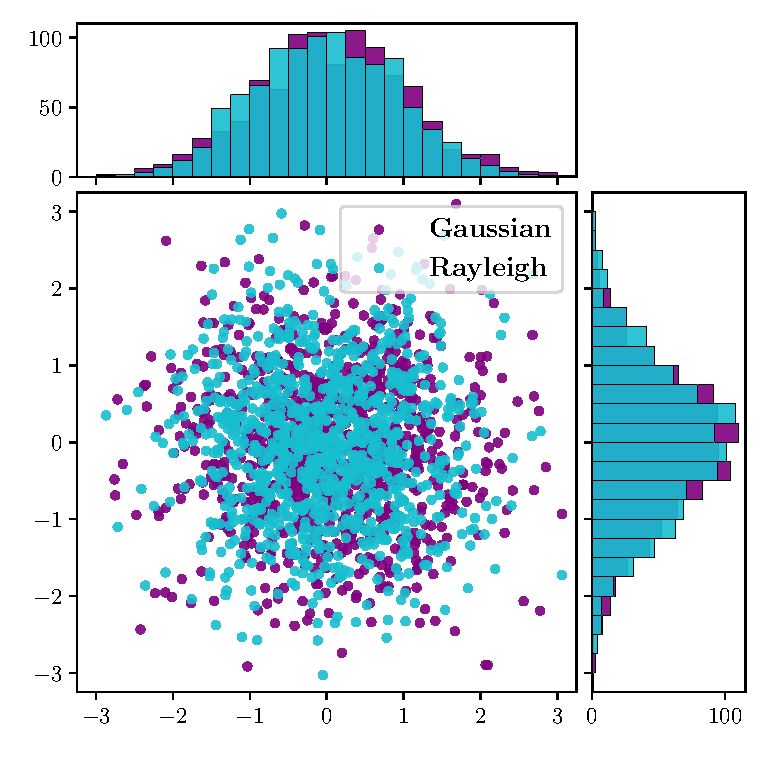
\includegraphics[width=\textwidth]{images/7_rayleigh.pdf}
    \caption{\label{fig:rayleigh} Sampling a 2D Gaussian against a Rayleigh distributed amplitude with uniform complex phase. In purple is the complex number $X+iY$ with $X,Y \sim \mathcal{N}(0,1)$, in cyan is $Re^{i\theta}$ with $R\sim\mathcal{R}(1)$ and $\theta \sim \mathcal{U}(0,2\pi)$.}
\end{figure}

\subsection{Lognormal field}
The universe today is not Gaussian. GRFs are able to capture the 2-point statistics of cosmological fields, but they cannot capture their skewed distribution. A possible way to get closer to the true distribution of the convergence field is with a lognormal transformation \cite{lognormal} \cite{lognormal2} \cite{lognormal3} \cite{fwdmodel}. In this work we will denote lognormal transformations as $\mathcal{L}$ and adopt the following convention for both the field and the correlation function,
\begin{gather}
    \label{eq:L_w}
    \mathcal{L}_w^{-1}(w^{L}, a) \equiv \log \left(\frac{w^{L}}{a^2}+1\right) = w^G,\\
    \label{eq:L_k}
    \mathcal{L}_\kappa(\kappa^G, a) \equiv a\left(\exp(\kappa^G-\tfrac{1}{2}\text{Var}(\kappa^G)) -1\right) = \kappa^{L}.
\end{gather}
Where the superscripts L and G respectively stand for lognormal and Gaussian, Var($\cdot$) stands for the variance of the field and $a$ is the so-called shift parameter, which is an indicator of the non-Gaussianity of the resulting field.

\section{Gaussian process}
\label{sec:gaussian process}
One way to think of Gaussian processes is as an extension of random vectors to infinite dimensions. Following this train of thought, let's begin with the concept of a random variable following a normal distribution. We say,
\begin{equation*}
    X \sim \mathcal{N}\left(\mu, \sigma^2\right),
\end{equation*}
to mean that $X$ is a sample of a Gaussian of mean $\mu$ and variance $\sigma^2$. If we were to get enough samples $X$, we would eventually recover its distribution. The generalisation of this concept to n-dimensions is a collection of random variables, described by a so-called multivariate normal distribution,
\begin{equation*}
    \bm{X} \sim \mathcal{N}\left(\bm{\mu}, \bm{K}\right).
\end{equation*}
Where $\bm{X}=(X_0,X_1,...)$ is a vector of random variables, $\bm{\mu}$ is the mean vector and $\bm{K}$ the covariance matrix. For a zero mean field, the covariance matrix is formed by the variance of each of the random variables on its diagonal, while the cross correlation terms populate the rest of the matrix. 
\subsection{Definition}
Adopting the philosophy of Rasmussen \cite{rasmussen}, functions can be thought of as very long vectors of the form $\left(f(x_1), f(x_2), ...\right)$. Such a view allows us to extend the definition of multivariate Gaussians, to functions. Defining $\mathcal{GP}$ a Gaussian process, a sample function $f$ will be given by:
\begin{equation}
    f(\bm{x}) \sim \mathcal{GP}\left(m(\bm{x}), k(\bm{x}, \bm{x'})\right)
\end{equation}
with $m(\bm{x})$ and $k(\bm{x}, \bm{x'})$ defined as,
\begin{gather}
    m(\bm{x})=\mathbb{E}[f(\bm{x})],\\
    k(\bm{x}, \bm{x'})=\mathbb{E}[(f(\bm{x})-m(\bm{x}))(f(\bm{x}')-m(\bm{x}'))],
\end{gather}
 Mathematically a GP is defined for a continuous function. Computationally this is not possible and we must treat space as a discrete grid. 

\subsection{Prior and posterior samples}
Given some $m(\cdot)$ and $k(\cdot,\cdot)$ which define a GP, a random sample from said GP would be a function $\bm{f}_*$ defined on a domain $D_*$, which is our grid.
\begin{equation}
    \bm{f}_* \sim \mathcal{N}(\bm{m}, \bm{K}_{**}).
    \label{eq:gp prior}
\end{equation}
Here we adopt the convention $\bm{K} = k(D_*,D_*)$. When drawing a sample function from \textit{Eq. }\eqref{eq:gp prior}, computationally the operation is equivalent to drawing a vector from a multivariate Gaussian. What we obtain is a so-called prior, or priors, see \textit{Fig. }\ref{fig:priors}.
\begin{figure}[h]
    \centering
    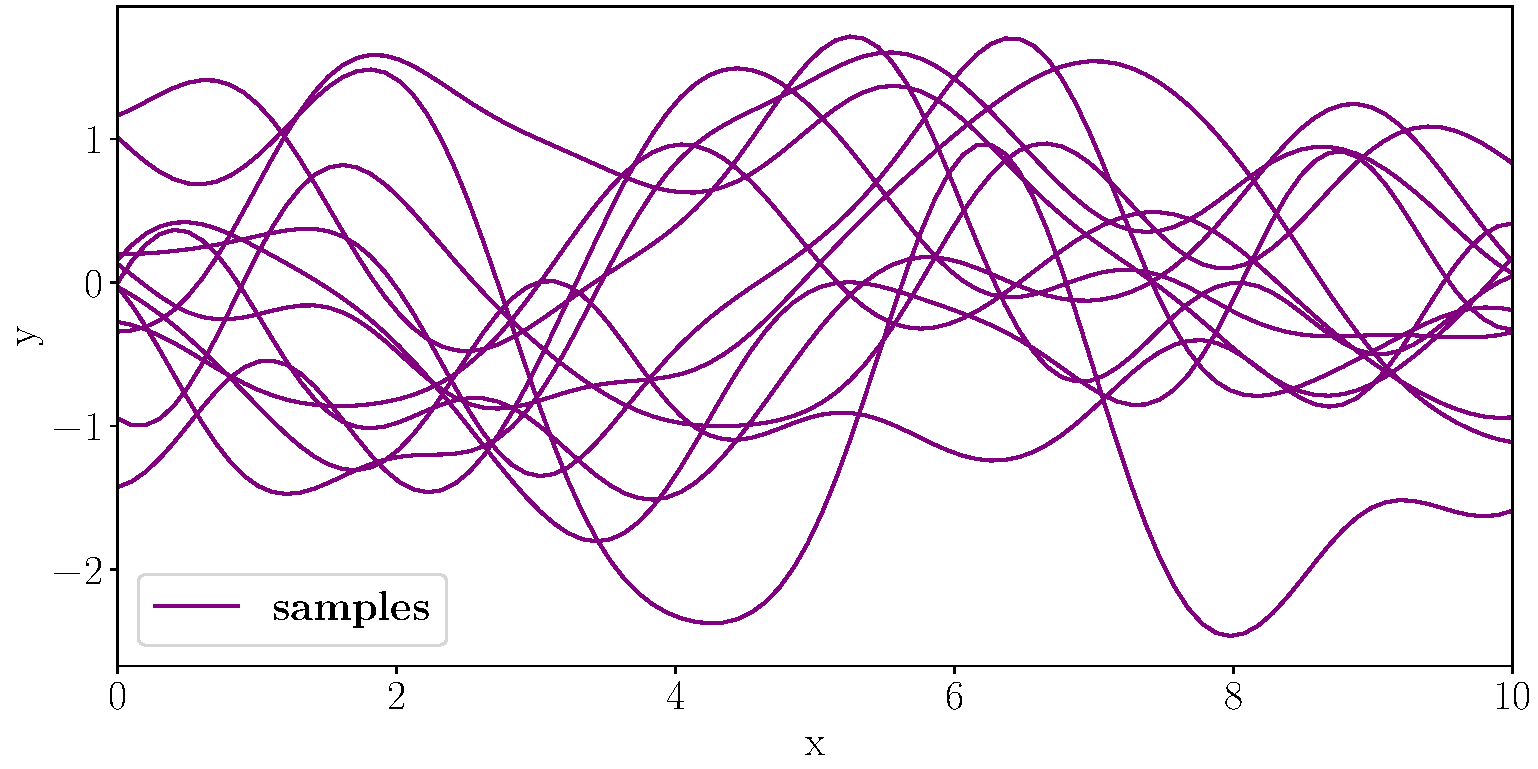
\includegraphics[width=\textwidth]{images/1_priors.pdf}
    \caption{Prior samples of a GP with mean $m(\bm{x})=0$ and squared exponential kernel $k(\bm{x},\bm{x'})=e^{-(\bm{x}-\bm{x'})^2}$.}
    \label{fig:priors}
\end{figure}

Let's now see how we can introduce knowledge of data points in this system. We divide the grid in training points $D$ and test points $D_*$. To each training point is associated a known value $\bm{y}$ and variance $\sigma_n^2$, whereas the values of the function at the test points $\bm{f}_*$ are unknown. We can summarise this as,
\begin{equation}
    \begin{bmatrix}
    \bm{y} \\
    \bm{f}_* \\
    \end{bmatrix}
    \sim \mathcal{N}\left(\bm{m}, \begin{bmatrix}
    \bm{K} + \sigma_n^2 I & \bm{K}_* \\
    \bm{K}^T_* & \bm{K}_{**} \\
    \end{bmatrix}\right)
\end{equation}
where we have once again adopted the notation $\bm{K}=k(D,D)$, $\bm{K_{*}}=k(D,D*)$, $\bm{K_{**}}=k(D_*,D_*)$. At this point, one way to find samples that follow the data would be to blindly draw priors until we get something that goes through all data points. This would be inefficient and computationally wasteful. Instead, we make a better guess for the test function values. This operation is called conditioning, because we condition the joint Gaussians on the training points, this gives
\begin{equation}
\bm{f}_* \mid D_*, D, \bm{y} \sim \mathcal{N}\left( \bm{K}^T_* [\bm{K} + \sigma_n^2 I]^{-1} \bm{y} , \bm{K}_{**} - \bm{K}^T_* [\bm{K} + \sigma_n^2 I]^{-1} \bm{K}_* \right).
\label{eq:conditioning}
\end{equation}
Conditioning can therefore give rise to what is called a posterior sample, \textit{Fig. }\ref{fig:posteriors}. The result is still a multivariate Gaussian, but the mean and variance given by \textit{Eq. }\eqref{eq:conditioning} generate samples that are a better guess of the behaviour of the function outside of the training points.
\begin{figure}[h]
    \centering
    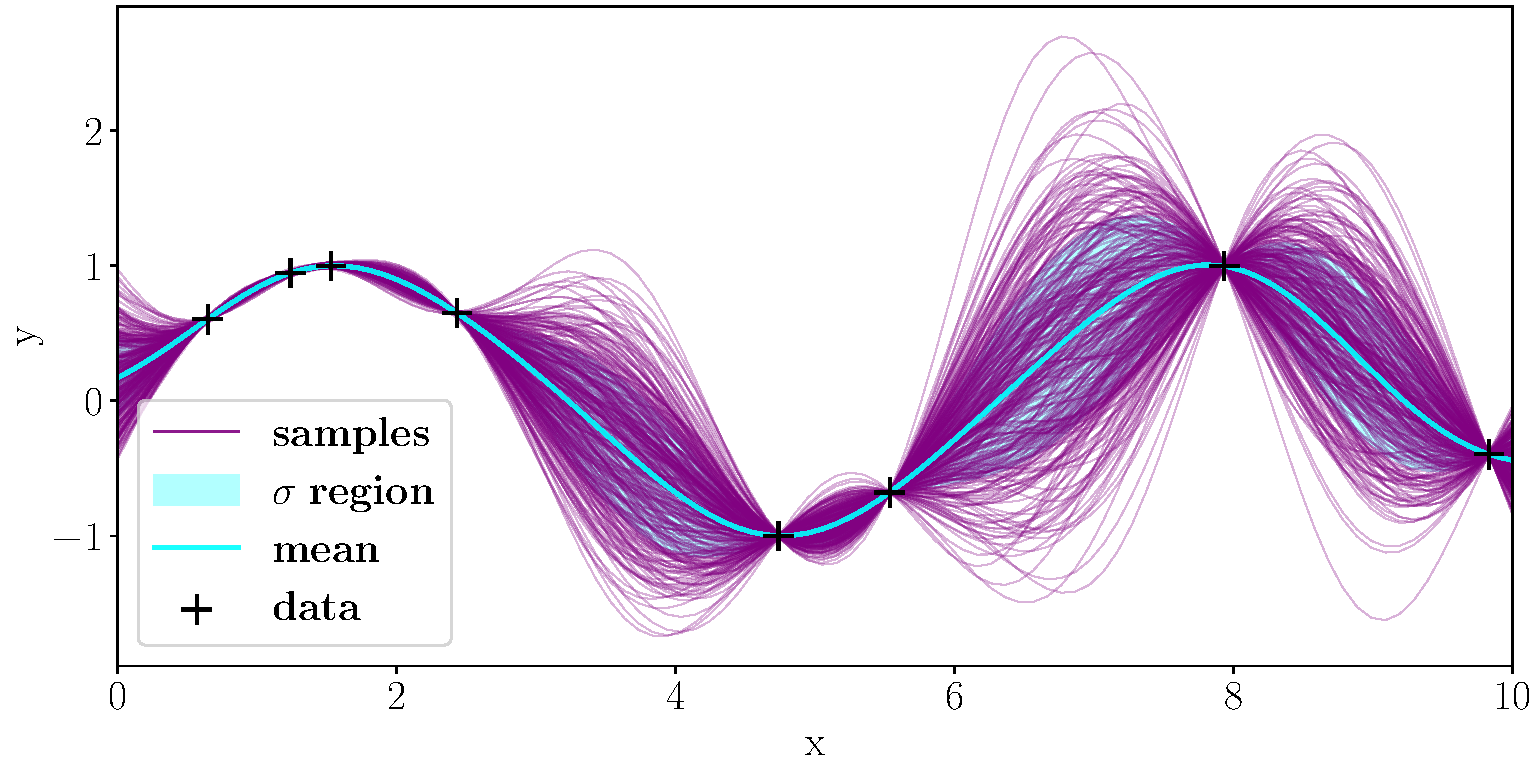
\includegraphics[width=\textwidth]{images/1_posteriors.pdf}
    \caption{\label{fig:posteriors} Summary plot of a GP conditioned to some data. The cyan line is the mean of the GP and the filled region corresponds to $1\sigma$. The purple lines are posterior samples, which are distributed Gaussianly around the mean. The data points are clearly marked in black, they are also the points where all samples converge to.}
\end{figure}

\begin{comment}
\subsection{Likelihood [should I include this?]}
The probability density function of the function values $\bm{f}$ under the Gaussian prior $\bm{f}\mid X \sim \mathcal{N}(\bm{0}, \bm{K})$ is
\begin{equation}
    p(\bm{f\mid X}) \propto \mid\bm{K}\mid^{-{\tfrac{1}{2}}} \exp\left(-{\tfrac{1}{2}} \bm{f}^\mathrm{T} \bm{K}^{-1} \bm{f}\right)
\end{equation}
or
\begin{equation}
    \log p(\bm{f\mid X}) \propto -{\tfrac{1}{2}}\log \mid\bm{K}\mid-{\tfrac{1}{2}} \bm{f}^\mathrm{T} \bm{K}^{-1} \bm{f}
\end{equation}
from here it can be shown that if the data $\bm{y}$ is normally distributed around some value $f$, meaning $\bm{y\mid f}\sim\mathcal{N}(\bm{f}, \sigma_n^2\bm{I})$, then by marginalising over all possible values of $\bm{f}$, we obtain
\begin{equation}
    \log \mathcal{L}(\bm{y\mid X}) \propto -{\tfrac{1}{2}}\log \mid\bm{K}+\sigma_n^2\bm{I}\mid-{\tfrac{1}{2}} \bm{y}^\mathrm{T} (\bm{K}+\sigma_n^2\bm{I})^{-1} \bm{y}.
\end{equation}
\end{comment}
%%%%%%%%%%%%%%%%%%%%%%%%%%%%%%%%%
%%%%%%%%%%%% CHAPTER %%%%%%%%%%%%
%%%%%%%%%%%%%%%%%%%%%%%%%%%%%%%%%
\chapter{Methods}

\section{Data simulation}
\label{sec:data simulation}
\subsection{Cosmology}
\label{subsec:cosmology}

\begin{wraptable}{r}{2.8cm}
%\vspace{-0.7cm}
\centering
\caption{\label{tab:fiducial_cosmology}Fiducial cosmology values given to \code{jaxcosmo}.}
%% Given these simple cosmological parameters, $S_8=\sigma_8\sqrt{\Omega_m/0.3}$ will take the value of $0.8$.
  \begin{tabular}{ll}
    \toprule
     & Fiducial \\
    \midrule
    $\Omega_m$ & 0.3 \\
    $\Omega_b$ & 0.05 \\
    $\Omega_k$ & 0 \\
    $h$ & 0.7 \\
    $n_s$ & 0.97 \\
    $\sigma_8$ & 0.8 \\
    $w_0$ & -1 \\
    $w_a$ & 0 \\
    \bottomrule
  \end{tabular}
\end{wraptable} 
This work follows in the general footsteps of data analysis of weak lensing surveys like \textit{HSC} \cite{cosmology:hsc} and \textit{KiDS} \cite{cosmology:kids450}\cite{cosmology:kids1000}, as we aim to replicate their methodologies.
Throughout the work, we assume a fiducial cosmology of fixed parameter values as shown in \textit{Tab. }\ref{tab:fiducial_cosmology}. In particular, all data maps will be generated from a power spectrum following this cosmology. We will refer to this power spectrum as the fiducial power spectrum $C(l)$. A leading modelling choice comes with the redshift distribution $n(z)$. We model it as a Smail-type distribution \cite{smail}\cite{smail2},
\begin{equation}
    n(z)=z^\alpha \exp{\left[-\left(\frac{z}{z_0}\right)^\beta\right]}.
\end{equation}
The choice of parameters has been made to emulate bin 5 of the \textit{KiDS1000} survey \cite{cosmology:kids1000_bins}, with parameters $\alpha=3.5$, $\beta=4.5$, $z_0=1$. 

\begin{figure}[h]
    \centering
    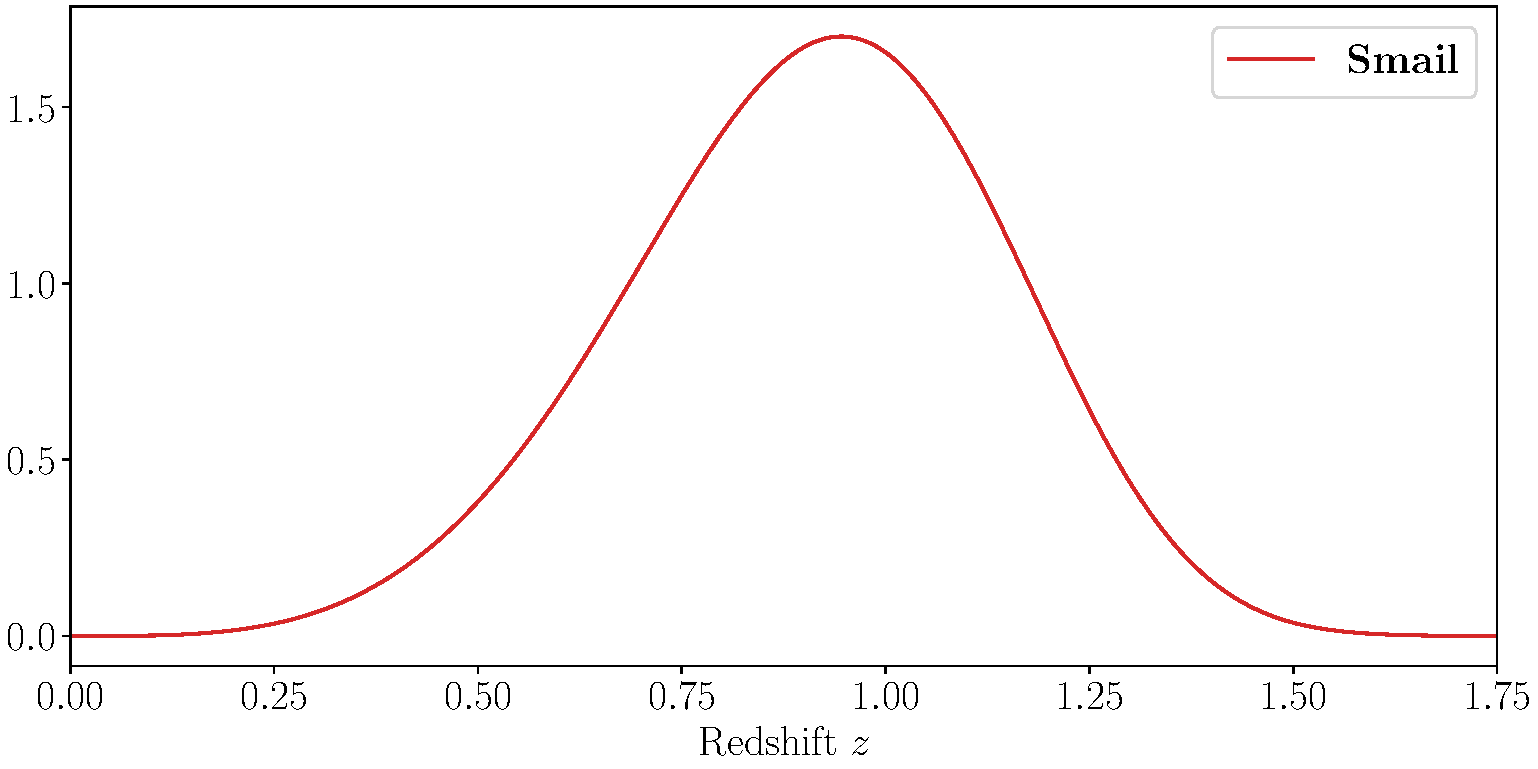
\includegraphics[width=\textwidth]{images/2_smail.pdf}
    \captionof{figure}{Smail-type redshift distribution for the chosen parameters: $\alpha=3.5$, $\beta=4.5$, $z_0=1$.}
    \label{fig:smail}
\end{figure}

\begin{comment}
"Omega_m": 0.3,
"Omega_b": 0.05,
"Omega_k": 0.0,
"h": 0.7,
"n_s": 0.97,
"S8": 0.8,
"w0": -1.0,
"wa": 0.0, 
\end{comment}

\subsection{Map making pipeline}
\label{sec:map making pipeline}
When dealing with maps of finite size $(L, L)$ and pixel resolution $(N,N)$, Fourier space is going to have boundaries, just as real space does. These limits are given by
\begin{gather*}
    l_{\text{min}} = \frac{2\pi}{L},\\
    l_{\text{max}} = \frac{2\pi}{L} N.
\end{gather*}
Therefore, a map of size $(10^{\circ},10^{\circ})$ and a grid $64\times64$ will have limits $(l_{\text{min}}, l_{\text{max}}) = (36, 2304)\text{rad}^{-1}$. Now that we have the physical range for the power spectrum, we can generate data.
\begin{figure}[h]
%\centering
\begin{tikzpicture}[>=stealth, node distance=2.5cm]
  % Nodes
  \node[diamond, draw=black, fill=black, text=white, minimum size=18mm, font=\Large, rounded corners] (a) at (0,0) {$C(l)$};
  \node[diamond, draw=black, fill=white, minimum size=18mm, font=\Large, rounded corners] (b) at (1.5,1.5) {$\tilde{w}^{L}$};
  \node[diamond, draw=black, fill=white, minimum size=18mm, font=\Large, rounded corners] (c) at (4,1.5) {$\tilde{w}^{G}$};
  \node[diamond, draw=black, fill=white, minimum size=18mm, font=\Large, rounded corners] (d) at (6.5,1.5) {$\tilde{C}^{G}$};
  \node[circle, draw=black, fill=white, text=black, minimum size=14mm, font=\Large, rounded corners] (e) at (8.9,1.5) {$\tilde{\kappa}^{G}$};
  \node[circle, draw=black, fill=black, text=white, minimum size=14mm, font=\Large, rounded corners] (f) at (11,1.5) {$\kappa^{L}$};
  \coordinate (g) at (1.3,-1.5);
  \node[circle, draw=black, fill=black, text=white, minimum size=14mm, font=\Large, rounded corners] (h) at (11,-1.5) {$\kappa^{G}$};

  % Arrows
  \draw[->, line width=1.5pt] (a) to[out=90, in=180, looseness=1.2] node[near end, above] {$\mathcal{H}^{-1}$} (b);
  \draw[-, line width=1.5pt] (a) to[out=270, in=180, looseness=1.2] (g);
  \draw[->, line width=1.5pt] (g) -- node[above] {\textit{GRF}} (h);
  \draw[->, line width=1.5pt] (e) -- node[above] {$\mathcal{L}_\kappa$} (f);
  \draw[->, line width=1.5pt] (b) -- node[above] {$\mathcal{L}_w^{-1}$} (c);
  \draw[->, line width=1.5pt] (c) -- node[above] {$\mathcal{H}$} (d);
  \draw[->, line width=1.5pt] (d) -- node[above] {\textit{GRF}} (e);
\end{tikzpicture}

\caption{Sequence of transformations used to generate Gaussian and lognormal maps starting from the fiducial angular power spectrum. The top branch shows how to generate a GRF which when transformed to a lognormal field, follows the fiducial $C(l)$.  The bottom branch is a standard GRF realisation starting from the fiducial $C(l)$. $L$ and $G$ stand for lognormal and Gaussian respectively. $\mathcal{H}$ is the Hankel transformation, and tilde refers to intermediate results.}
\label{tik:cw}
\end{figure}

To generate a GRF, we employ the algorithm mentioned in \textit{Eq. }\eqref{eq:grf 2D}. However, in making a lognormal field, the matter is a bit more complicated. Any GRF on which we apply the lognormal transformation $\mathcal{L}_\kappa$, from \textit{Eq. }\eqref{eq:L_k}, becomes a lognormal field. The reason we do not just lognormal transform any field is given by the fact that they would not recover the fiducial power spectrum $C(l)$. Our goal is therefore to find a transfer GRF $\tilde{\kappa}^G$ which, when transformed lognormally, gives rise to a lognormal field $\kappa^L$ that recovers $C(l)$. To do so, we follow the sequence of transformations illustrated in the top branch of \textit{Fig. }\ref{tik:cw}.

\subsection{Noise and mask}
\begin{figure}[h]
    \centering
    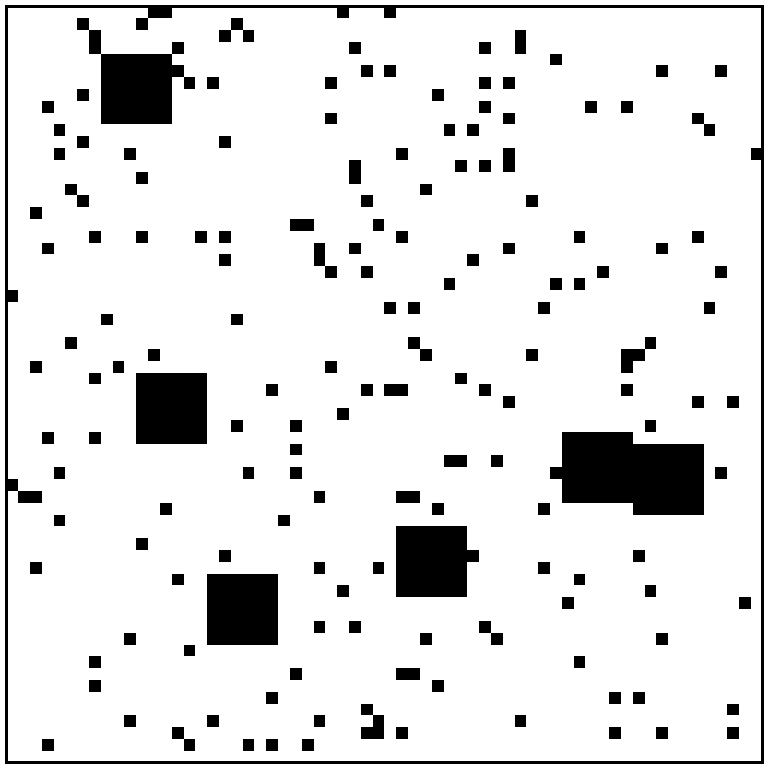
\includegraphics[width=0.5\linewidth]{images/5_random_and_blocks_mask.pdf}
    \caption{Approximately $10\%$ mask applied to the data. Size $(10^{\circ},10^{\circ})$ and grid $64\times64$.}
    \label{fig:mask}
\end{figure}
As all data is being simulated, we only take into account the so-called shape noise, which is due to the intrinsic distribution of ellipticities and angle formed with respect to us. GPs will treat each pixel of the map as a random variable Gaussianly distributed with standard deviation given by \cite{noise},
\begin{equation}
    \sigma_\text{noise} = \frac{\sigma_e}{\sqrt{n_g A_{px}}}.
    \label{eq:noise}
\end{equation}
We use values of $\sigma_e=0.26$, $n_g= 4, 10, 30, 100 \text{ galaxies}/\text{arcmin}^2$, and a pixel area given by the pixel resolution squared, $A_{px}=(L/N)^2$. For our highest-resolution run, we have $N=64$ and use $n_g = 10 \text{ galaxies}/\text{arcmin}^2$, which results in a noise standard deviation of $\sigma_\text{noise} \sim 0.0088$. The mask being used as seen in \textit{Fig. }\ref{fig:mask}, covers approximately $10\%$ of the patch \cite{pixel}. We keep the noise and mask random seeds fixed throughout the work.

\section{Kernel}
\label{sec:gaussian process kernel}
The kernel of a Gaussian process is given by a function of the form $k(x,y)$. It takes in two points, $x$ and $y$, and returns the value of their correlation. In our case, specifically, $x$ and $y$ will be two points in a grid of shape $(N,N)$, and the kernel function will be the convergence angular autocorrelation function. As all code used for this paper is written in \code{JAX} \cite{jax} we opt for the use of the library \code{tinygp} \cite{tinygp} for all Gaussian process computations. \code{tinygp} allows for the use of a custom kernel with a custom \code{evaluate} method, which takes two points on the grid and returns the correlation value. We follow with two \code{Python} pseudocodes of our kernel implementations.
\begin{lstlisting}[language=Python, label={lst:hankel}, caption=\code{kernel_Hankel} uses the helper function \code{Hankel} which returns a 1D callable correlation function \code{w}. Then finds the euclidean distance between $x$ and $y$ and evaluates the correlation function at that point. We will discuss how we perform the Hankel transformation in the following section.]
class kernel_Hankel:
    def __init__(self, cl, N, L):
        self.w   = Hankel(cl, N, L)
        self.r   = L / N
        
    def evaluate(self, x, y):
        theta    = self.r * sqrt(sum(x - y))
        return self.w(theta)
\end{lstlisting}
 
\begin{lstlisting}[language=Python, label={lst:FFT}, caption=\code{kernel_FFT} performs a 2D Fourier transform on the power spectrum \code{cl2D}. This returns a 2D array that is the correlation function. Then to evaluate \code{w2D} we need two indices. These are given by the difference of $x$ and $y$ component wise. Furthermore we have to be careful about possible mismatches between the shape of \code{cl2D} and the grid of our map. For this we have the renormalisation factor \code{r}. We will discuss further how we get \code{cl2D} in the following section.]
class kernel_FFT:
    def __init__(self, cl2D, N, L):
        M        = sqrt(cl2D.size)
        self.w2D = abs(ifft2(cl2D)) * M**2 / L**2
        self.r   = M / N
        
    def evaluate(self, x, y):
        d0       = self.r * abs(x[0] - y[0])
        d1       = self.r * abs(x[1] - y[1])
        return self.w2D[int(d0)][int(d1)]
\end{lstlisting}

\subsection{Hankel transform}
\label{sec:Hankel transform}
In order to build a Gaussian process kernel, we need to find the correlation function that best describes the data. The way we do this is by computing the angular power spectrum and transforming it in the corresponding angular correlation function. Let's explore the previously discussed flat-sky relation between angular power spectrum and correlation function given by \textit{Eq. }\eqref{eq:flatsky hankel}. This particular integral of a Bessel function is also known as a zeroth order Hankel transformation,
\begin{equation}
    w(\theta) = \int \frac{dl}{2\pi} l C(l) J_0(l\theta).
    \label{eq:C-w hankel}
\end{equation}
We will explore two methods for computing this integral: the \textit{integration} method \textit{Sec. }\ref{sec:integration method} and the \textit{FFTlog} method \textit{Sec. }\ref{sec:FFTlog method}.

\subsubsection{Integration}
\label{sec:integration method}
Integration is the most straight forward way to evaluate the integral, but it requires to implement an algorithm for the approximation of the Bessel function $J_0$. The advantages of this method:
\begin{itemize}
    \item it is easy to integrate over the correct $l$-range, from $l_{\text{min}}$ and $l_{\text{max}}$, a freedom that we do not have with the FFTlog.
\end{itemize}
The disadvantages:
\begin{itemize}
    \item integration is computationally slow, especially when dealing with highly oscillatory behaviour introduced by the Bessel function, which requires fine sampling.
\end{itemize}

\subsubsection{FFTlog}
\label{sec:FFTlog method}
The FFTlog method \cite{fftlog} is a fast implementation of the Hankel transformation. In fact it simplifies \textit{Eq. }\eqref{eq:C-w hankel} by assuming a power decomposition of $C(l)$. Such a decomposition is achievable by taking the \textit{fast Fourier transformation (FFT)} in $\log k$, hence the name FFTlog. The power spectrum becomes,
\begin{equation}
    C(l)=\sum_\alpha c_\alpha l^{\upsilon + i\eta_\alpha}.
\end{equation}
Substituting in \textit{Eq. }\eqref{eq:C-w hankel},
\begin{equation*}
    w(\theta) = \sum_\alpha c_\alpha \int_0^\infty \frac{dl}{2\pi} l^{\upsilon + i\eta_\alpha+1} J_0(l\theta).
\end{equation*}
Take $x=l\theta$ and $s_\alpha-1=\upsilon + i\eta_\alpha+1$,
\begin{equation*}
    w(\theta) = \sum_\alpha c_\alpha \theta^{-s_\alpha} \int_0^\infty \frac{dx}{2\pi} x^{s_\alpha-1} J_0(x).
\end{equation*}
Lastly we recognise $\int_0^\infty dx x^{s-1}J_0(x) = \frac{2^{s-1}}{\pi}\sin(\pi s/2) [\Gamma(s/2)]^2$, a Mellin transform. Using this tabulated result we conclude that the correlation is given by the sum,
\begin{equation}
    w(\theta) = \frac{1}{2\pi^2}\sum_\alpha c_\alpha \theta^{-s_\alpha}2^{s_\alpha-1}\sin(\pi s_\alpha/2) [\Gamma(s_\alpha/2)]^2.
\end{equation}
For the Mellin transform identity to hold analytically, the integral bounds have to go from 0 to $\infty$. Although computationally we don't need to consider such a wide range, we still have to broaden the integration limits to something larger than our $l$-range; so as to avoid ringing effects. Experimentally we have found that extending the $l$-range between $l_{\text{min}}/4$ and $l_{\text{max}}$, is enough to compensate for such effects. The advantages of this method:
\begin{itemize}
    \item the FFTlog method is ultimately much faster than the integration method.
\end{itemize}
The disadvantages:
\begin{itemize}
    \item the widening of the $l$-range needed to avoid ringing effects inevitably adds power to the correlation function resulting in a higher variance and overall amplitude.
\end{itemize}

\subsection{Fourier transform}
The second transformation that we can use to go from power spectrum to correlation function, is the Fourier transformation discussed in \textit{Eq. }\eqref{eq:flatsky fft}. It is a more fundamental relation than the Hankel transformation as it does not assume that $l$ is radially symmetric. In our case, low resolution, coupled with a square map, means that the radial assumption might not apply. Note that, the lowest resolution grid we use is $32\times32$, with $L/N \sim 19$ arcmin; which is one order of magnitude worse than today's weak lensing data, around $\sim 3$ arcmin according to \cite{fwdmodel}.  In the following \textit{Sec. }\ref{sec:gaussian process kernel} we will find experimentally that the Hankel methods described above do not work well with our GP setup. For this reason, we explore this method of conversion between angular power spectrum and correlation function,
\begin{equation}
    w(\theta)=\int\frac{d^2l}{4\pi^2}e^{-i\bm{l}\cdot\bm{\theta}}C(l).
    \label{eq:C-w fft}
\end{equation}
As computers can only deal with discrete functions, it is important to note that we will be performing a \textit{discrete Fourier transformation (DFT)}. We will use the widely known FFT algorithm to compute DFTs. In particular we use JAX's implementation of the 2D FFT algorithm, \code{jax.numpy.fft.ifft2}. 

Let us find the relation between continuous Fourier transformation and DFT. The definitions of continuous and discrete Fourier transformations in 1D, are respectively:
\begin{align} 
    \mathcal{F}^{-1}&=\int\frac{dk}{2\pi}e^{ikx}, \label{eq:F}\\
    \text{F}^{-1}&=\frac{1}{N}\sum_p e^{ik_px}. \label{eq:DFT}
\end{align}
First of all, a DFT is dimensionless. Secondly, it is discrete and bounded. We can therefore rewrite \textit{Eq. }\eqref{eq:F} using the substitution $k(p)=2\pi \frac{p}{L}$ to discretise k-space,
\begin{equation*}
     \int\frac{dk}{2\pi}e^{ikx} = \int\frac{dp}{L} e^{ik(p)x} = \frac{1}{L}\sum_p e^{ik_px}.
\end{equation*}
Applying the definition of DFT as seen in \textit{Eq. }\eqref{eq:DFT}, it follows that in 1D
\begin{equation}
    \mathcal{F}^{-1}=\frac{N}{L}\text{F}^{-1}.
\end{equation}
Which means that the correlation function is given by a \textit{backwards} normalised inverse DFT to be scaled by a factor $(N/L)^d$, where $d$ is the dimension of the considered space. In our case, $d=2$. 

In order to perform a FFT in 2D, we will need a two dimensional extension of the angular power spectrum. We make use of its radial symmetry with respect to $\bm{l}=(l_x,l_y)$ and create a 2D grid of shape $(M,M)$ as shown in \textit{Fig. }\ref{tik:1D to 2D}. 
\begin{figure}[h]
\centering
\begin{tikzpicture}
  % Nodes
  \node[diamond, draw=black, fill=black, text=white, minimum size=18mm, font=\Large, rounded corners] (a) at (0,0) {$C^{1D}$};
  \node[diamond, draw=black, fill=black, text=white, minimum size=18mm, font=\Large, rounded corners] (b) at (5,0) {$C^{2D}$};

  % Arrows
  \draw[->, line width=1.5pt] (a) -- node[above] {$l \equiv \sqrt{l_x^2+l_y^2}$} (b);
\end{tikzpicture}
\caption{1D to 2D extension of the power spectrum $C(l)$}
\label{tik:1D to 2D}
\end{figure}
Now that we have a 2D power spectrum we can take the inverse two dimensional fast Fourier transformation to obtain a 2D correlation function. In practice, we will test two grids, which we name \textit{full-range FFT} method and \textit{half-range FFT} method. 
\subsubsection{Full-range FFT}
The full-range FFT is defined by a grid of shape $(2N,2N)$. Since the grid is radial, it will be centered. This implies that if we want to keep information of all $N$ modes,
\begin{equation}
    \frac{2\pi}{L},\, \frac{4\pi}{L},\,\cdot\cdot\cdot\,,\, \frac{2\pi}{L}N,
\end{equation}
the grid will have to be at least of shape $M=2N$.
The advantages of this method:
\begin{itemize}
    \item it keeps information on the full range of modes.
\end{itemize}
The disadvantages:
\begin{itemize}
    \item it introduces rounding errors, as the field has shape $(N,N)$ and not all of the possible distance combinations of such a grid are covered bya grid of shape $(2N,2N)$.
\end{itemize}
\subsubsection{Half-range FFT}
The half-range FFT is defined by a grid of shape $(N,N)$.
The advantages of this method:
\begin{itemize}
    \item has the perk of having no shape mismatch between field and correlation function.
\end{itemize}
The disadvantages:
\begin{itemize}
    \item it loses half of the $l$-range, missing information on small scales.
\end{itemize}
%%%%%%%%%%%%%%%%%%%%%%%%%%%%%%%%%
%%%%%%%%%%%% CHAPTER %%%%%%%%%%%%
%%%%%%%%%%%%%%%%%%%%%%%%%%%%%%%%%
\chapter{Results}

\section{Power spectrum recovery}
\subsection{Gaussian and lognormal fields}
\label{sec:gaussian and lognormal fields}
We begin by testing the consistency of our Gaussian and lognormal maps generation pipeline. 
\begin{figure}[h]
    \centering
    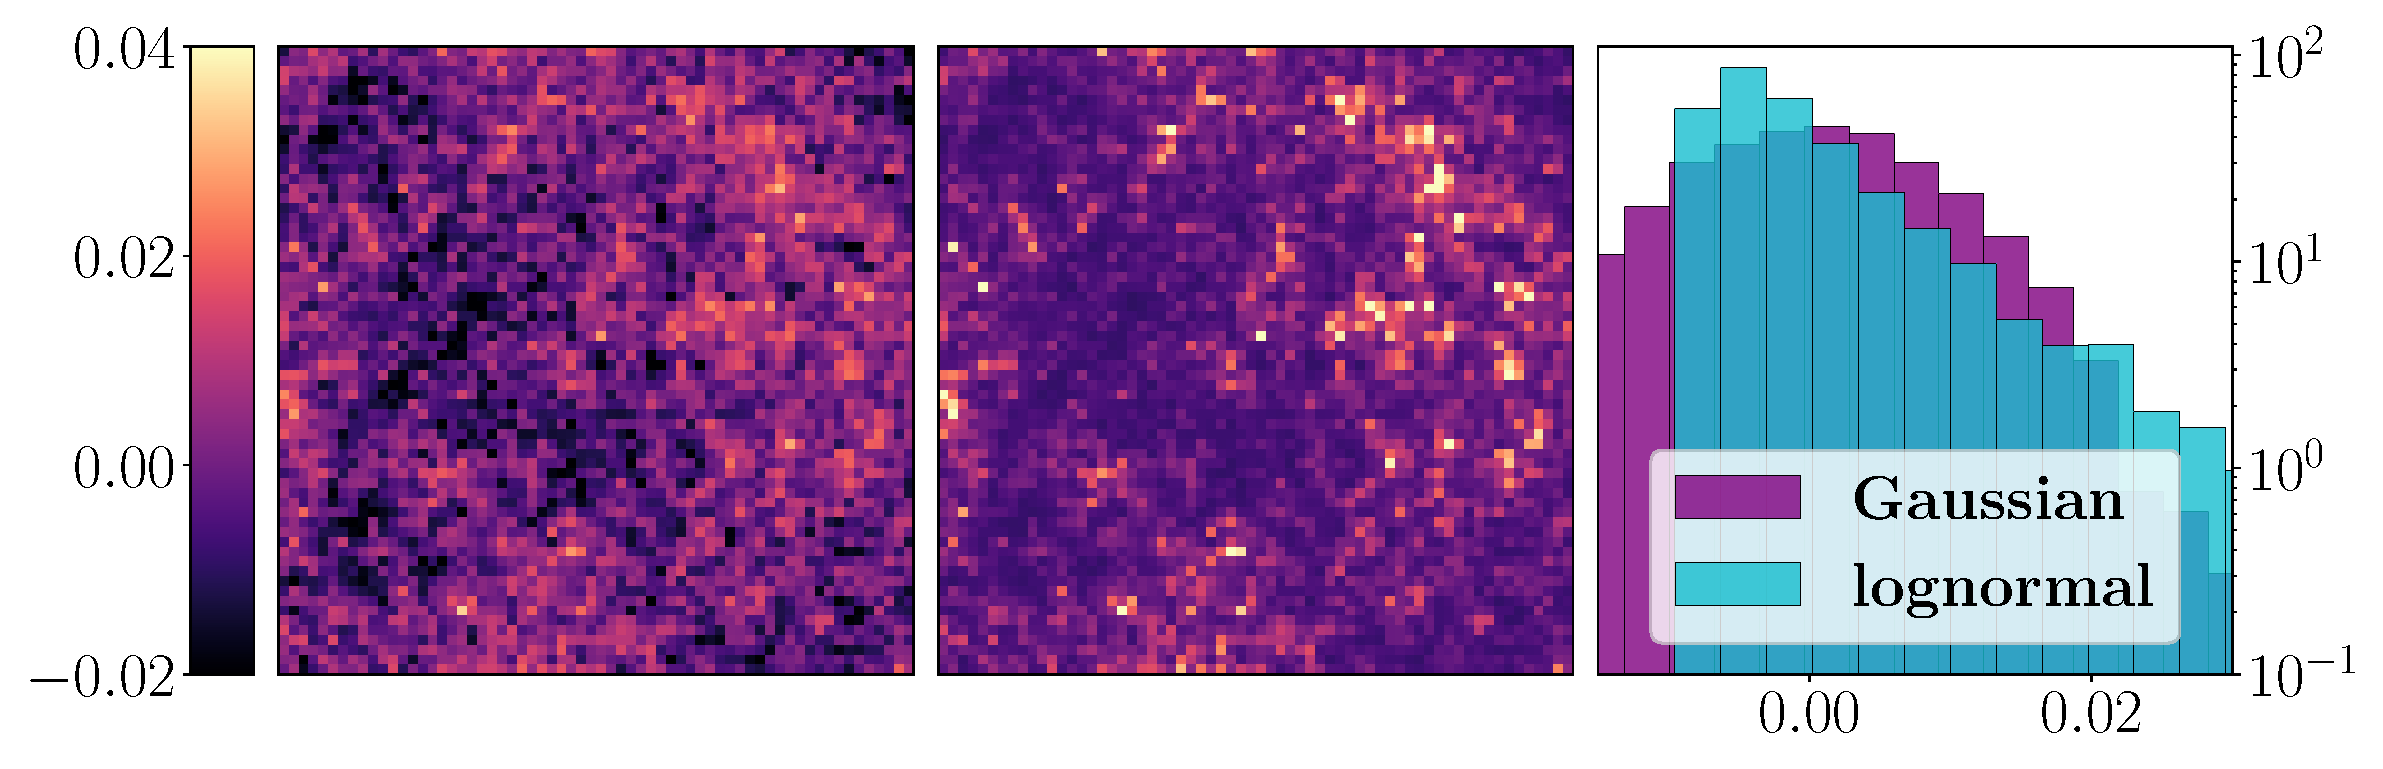
\includegraphics[width=1\textwidth]{images/4_Gaussian_lognormal_dist.pdf}
    \caption{\label{fig:fields dist} Comparison of a Gaussian map, on the left, with a lognormal map on the right. Both maps arise from the same random seed. The colorbar has been adjusted to enhance the differences between the two. The histogram plot shows the clear difference in the map distributions.}
\end{figure}

We show example realisations of the two fields in \textit{Fig. }\ref{fig:fields dist}, Gaussian on left and lognormal on the right. There's a visible difference between the two, as it can be seen clearly from the distribution plot. The main check to perform is for testing whether the generated fields recover the theoretical power spectrum. \textit{Fig. }\ref{fig:check fields} shows that this is the case for the Gaussian fields. They recover the fiducial $C(l)$ within a few percent error, with larger deviations $\sim 5\%$ at the low and high ends of the $l$-range. Instead, lognormal fields present deviations $\gtrsim 10\%$. As the lognormal transformations we use have been reported by different sources \cite{fwdmodel}\cite{lognormal}, the issue must lie with our \code{JAX} implementation of the Hankel transformation. Resolving such issues could be achieved by future iterations of this work. In this work, we restrict ourselves to the use of Gaussian fields, as it is enough to prove our thesis and show that Gaussian processes can be applied to cosmological fields.
\begin{figure}[h]
    \centering
    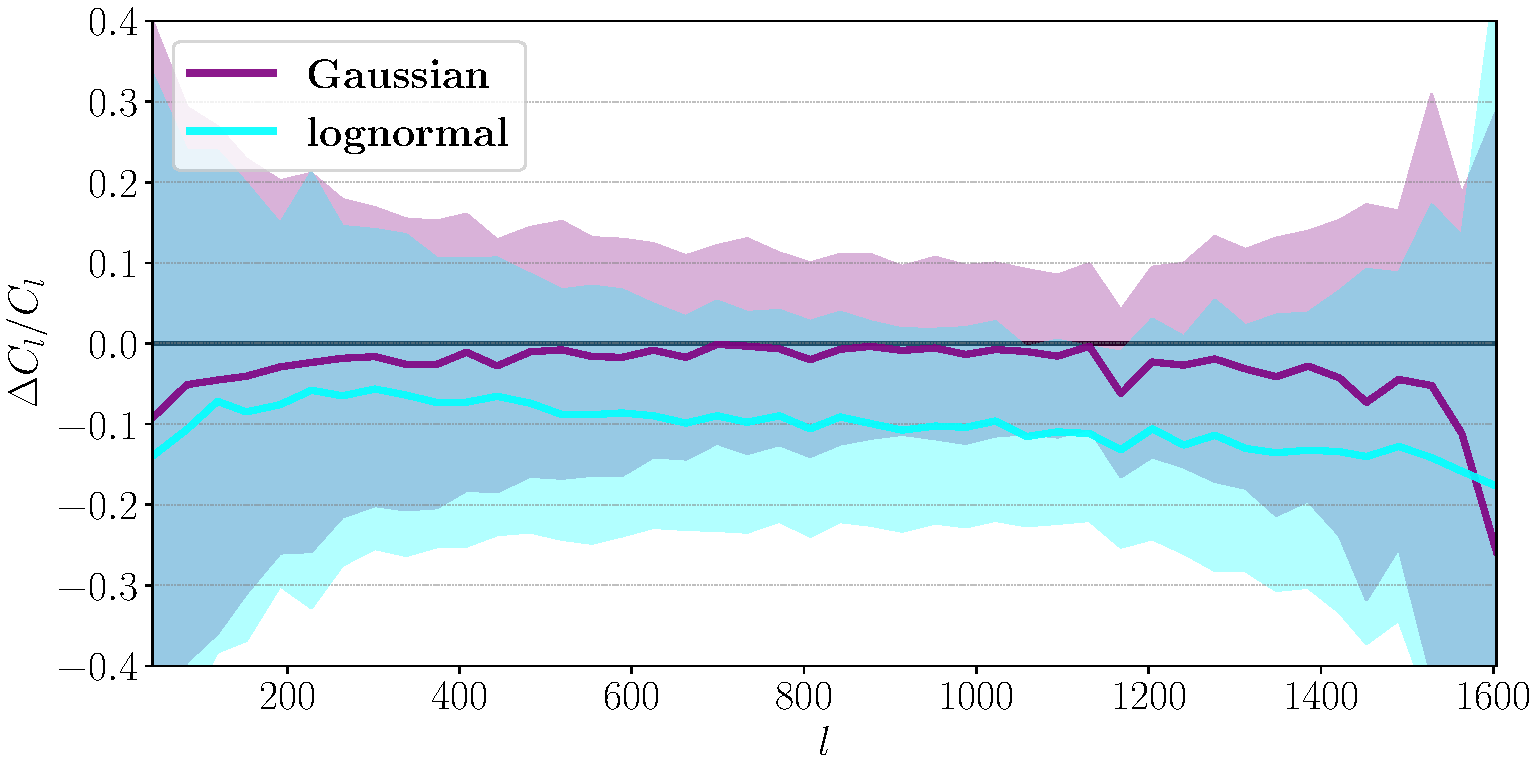
\includegraphics[width=1\textwidth]{images/4_Gaussian_lognormal_check.pdf}
    \caption{\label{fig:check fields} Power spectrum estimation from  Gaussian and lognormal maps. Mean and standard deviation are calculated with 500 realisation of both fields.}
\end{figure}

\subsection{Gaussian process priors}
\label{sec:gaussian process priors}
First, we test the ability of the kernels we have built in \textit{Sec. }\ref{sec:gaussian process kernel} to recover the power spectrum of our cosmology.  
\begin{figure}[h]
    \centering
    %\textit{Kernels comaprison}}\par
    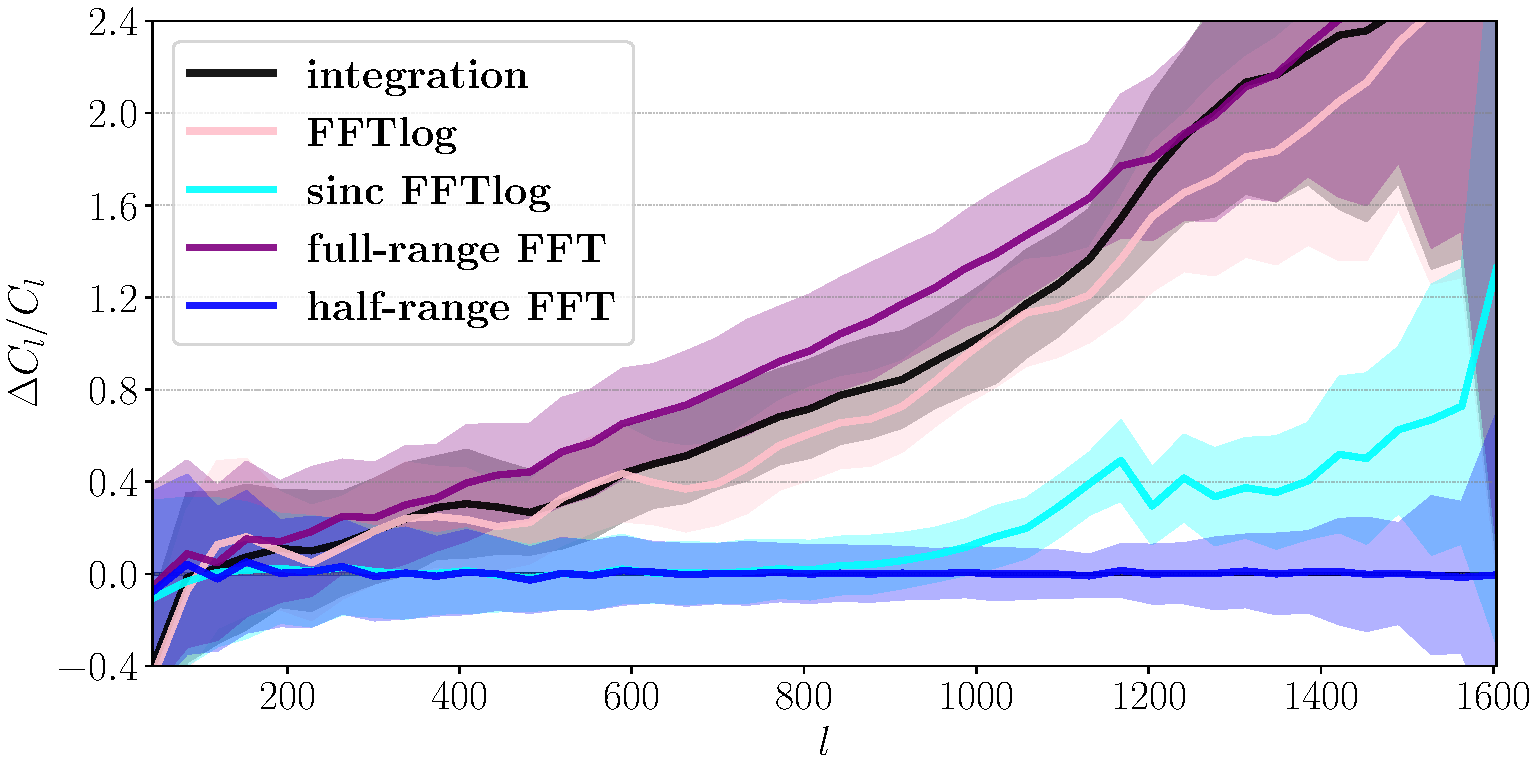
\includegraphics[width=\textwidth]{images/3_kernel_comparison.pdf}
    \caption{\label{fig:check methods} Reconstructed power spectrum from prior sample of GP with the four proposed kernels: integration, FFTlog, full-range FFT, half-range FFT and sinc FFTlog. Mean and standard deviation are calculated with 500 prior samples from each GP. }
\end{figure}
We test five models in \textit{Fig. }\ref{fig:check methods}: integration, FFTlog, full-range FFT, half-range FFT and sinc FFTlog. The first four methods are described in the Gaussian process kernels \textit{Sec. }\ref{sec:gaussian process kernel}, whereas the sinc FFTlog referes to a FFTlog model on which we applied smoothing, by multiplying the power spectrum by a factor of $sinc^4(l\frac{L}{2\pi N})$. The recovered power spectra are plotted against the fiducial power spectrum, or smoothed power spectrum for the sinc FFTlog. Mean and standard deviation associated to the plots are calculated from 500 samples. As expected the integration, FFTlog and full-range FFT perform similarly, as they all contain the same ammount of information. As these models deviate so strongly from the fiducial power spectrum we tried applying smoothing, which helps to recover half of the $l$-range at large scales. The only method that seems to be consistently recovering the fiducial power spectrum is the half-range FFT. One could argue that due to the inherent discreteness and boundedness of the fields we are working with, using FFTs is the most natural choice; also, half-range FFT uses the only grid that recovers a correlation function of the same shape as the field without having to perform binning.
\begin{figure}[h]
    \centering
    %\textit{Cosmology invariance}}\par
    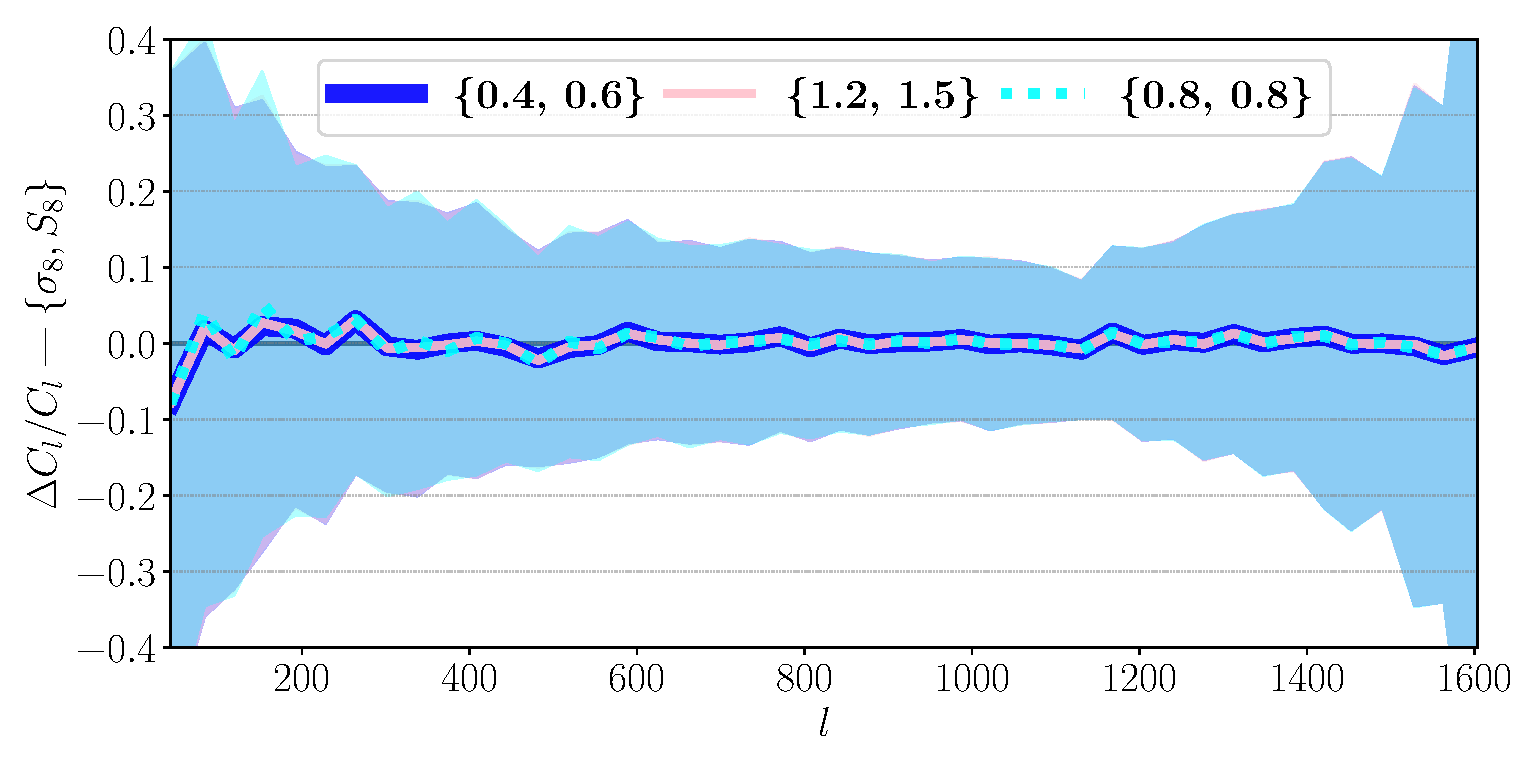
\includegraphics[width=\textwidth]{images/3_cosmology_comparison.pdf}
    \caption{\label{fig:check cosmology} Reconstructed power spectrum from prior samples of a GP, as a function of $\{\sigma_8, S_8\}$. Mean and standard deviation are calculated with 500 prior samples for each different cosmology.}
\end{figure}

We have also tested the efficacy of the half-range FFT model for different cosmologies of values $\{\sigma_8, S_8\}$ equal to $\{0.4,0.2\}$, $\{1.2,1.5\}$ and, our fiducial cosmology, $\{0.8,0.8\}$. As \textit{Fig. }\ref{fig:check cosmology} shows, the model is independent of the choice of cosmology. From here on the results will be presented assuming a kernel built with the half-range FFT model.

\section{Gaussian process map reconstruction}
\label{sec:gaussian process map reconstruction}
Armed with a reliable kernel, let's embark upon the journey of reconstructing a heavily masked cosmological field. What we will do is: create a noiseless GRF in the fiducial cosmology \textit{Tab. }\ref{tab:fiducial_cosmology}, \textit{True} map; apply a mask to obtain the \textit{Data} map; condition a Gaussian process which assumes the fiducial cosmology. \textit{Fig. }\ref{fig:GP reconstruction summary} lists the result of this operation, showing the resulting mean $\mu$ and standard deviation $\sigma$ of the conditioned GP. We also plot the ratio between residuals $\Delta=\mu-$\textit{True} and standard deviation squared, to test the goodness of fit of our model, the values of the map sum up to $\chi^2 \sim 2495$. With the mask covering $\nu=2353$ pixels, we obtain $\chi^2 / \nu = 1.06$. Of course, this is just a noiseless application, which is unreasonable for a real application.
\begin{figure}[h]
    \centering
    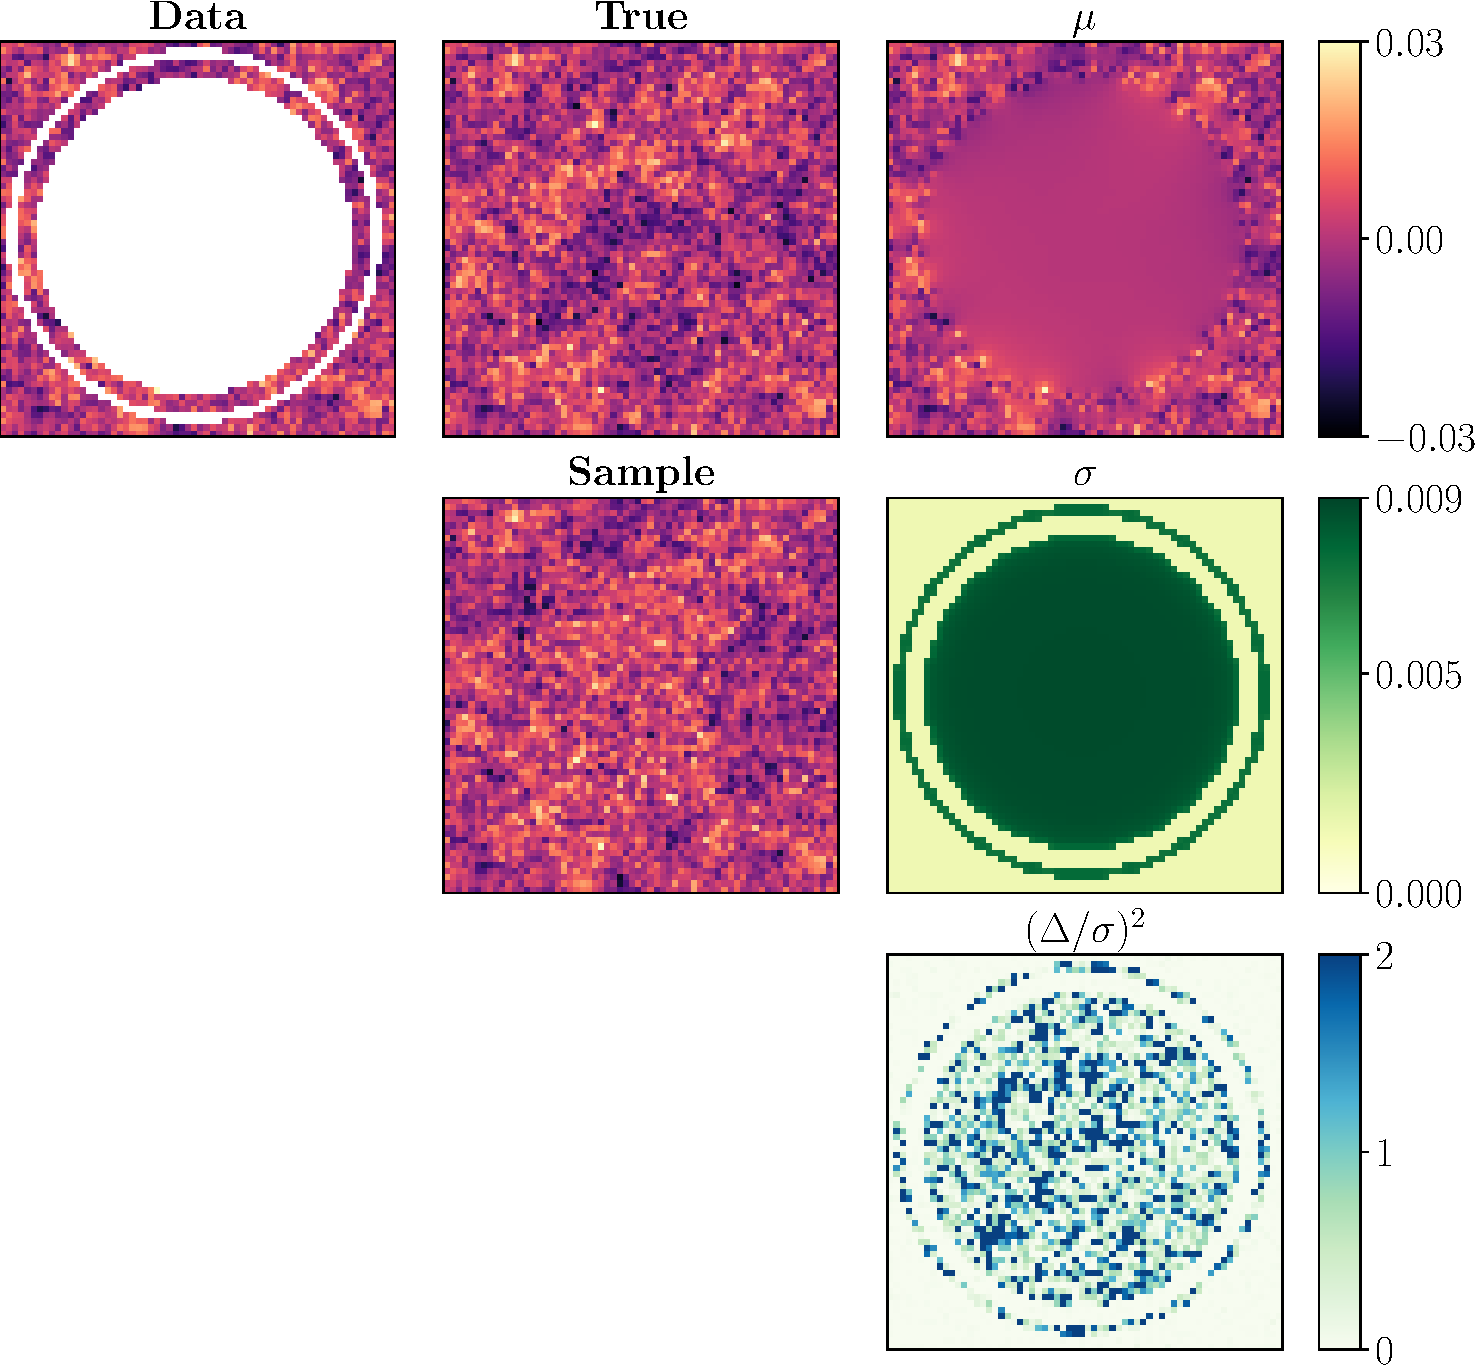
\includegraphics[width=\textwidth]{images/2_summary.pdf}
    \caption{\label{fig:GP reconstruction summary}Summary of field reconstruction abilities of a Gaussian process conditioned on data. The left column shows the masked GRF, which is our data. The middle column shows the true GRF without masks and a posterior sample drawn from the conditioned GP. The right column shows maps of the mean, standard deviation and residuals over standard deviation squared of the conditioned GP. Regions of higher uncertainty correspond to the masked regions. The residuals over standard deviation map also shows how regions with low mask recover the data.}
\end{figure}

\section{Inference of cosmological parameters}
\label{sec:inference of cosmological parameters}
To test the ability of Gaussian processes to recover cosmological parameters without any prior knowledge except a noisy and masked map, we perform a MCMC simulation to infer the posterior distributions of $\sigma_8$ and $S_8$. We use the convention 
\begin{equation}
    S_8 = \sigma_8 \sqrt{\frac{\Omega_m}{0.3}},
    \label{eq:S8}
\end{equation}
\begin{wraptable}{l}{3.7cm}
\centering
\caption{Priors used by our \code{numpyro} model for cosmological parameter inference}\label{tab:priors}
\begin{tabular}{ll}
    \toprule
     & Prior \\
    \midrule
    $S_8$ & $\mathcal{U}[0.565,1.78]$ \\
    $\sigma_8$ & $\mathcal{U}[0.4,1]$ \\
    $\Omega_m$ & $\mathcal{U}[0.15,0.95]$ \\
    \bottomrule
\end{tabular}
\end{wraptable} 
to infer deterministically a posterior for $\Omega_m$. Such a reparametrisation is needed due to the strong degeneracy between $\sigma_8$ and $\Omega_m$. \textit{Eq. }\eqref{eq:S8} breaks this degeneracy, changing the geometry of the sampling space and making the sampling more consistent. The model assumes uninformed flat priors for the cosmological parameters, as shown in \textit{Tab. }\ref{tab:priors}, such prior bounds are also in accordance with the \code{jaxcosmo} release \cite{jaxcosmo}. The likelihood of the model is given by a Gaussian process distribution conditioned on \textit{Data}, with a standard deviation equal to the noise applied to the map. The analysis is coded with \code{numpyro} \cite{numpyro} \cite{numpyro2}, using a the \textit{No-U-Turn Sampler (NUTS)} method with \code{max_tree_depth=16}, \code{target_accept_prob=0.8}. We simulate 8 chains for the $32\times32$ grid and 4 chains for the $64\times64$. Each chain performs 1000 warmup steps and 3000 samples. 


\subsection{One parameter}
As a first step and for a consistency check, we run the inference model for one cosmological parameter, keeping all others fixed. Using a $64\times64$ grid with $n_g=10 \text{ galaxies}/\text{arcmin}^2$. In \textit{Fig. }\ref{fig:MCMC one parameter} we show the inferred distribution for both $\sigma_8$ and $\Omega_m$. We find that we are able to recover the true value for both parameters within two sigmas, $\sigma_8 = 0.776\pm0.015$ and $\Omega_m = 0.284\pm0.010$. We notice a slight tendency of the inferred distribution to be biased low; a tendency we also observe next for both sampled parameters, $S_8$ and $\sigma_8$.
\begin{figure}[h]
    \begin{minipage}[b]{0.48\textwidth}
        \centering
        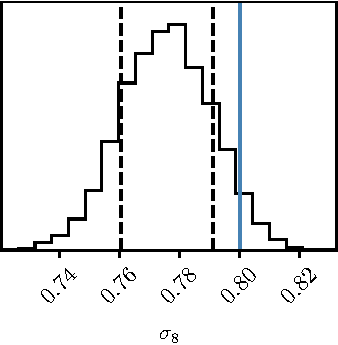
\includegraphics[width=\textwidth]{images/6_MCMC_sigma_parameters.pdf}
    \end{minipage}
    \hfill % Add horizontal space between minipages
    \begin{minipage}[b]{0.48\textwidth}
        \centering
        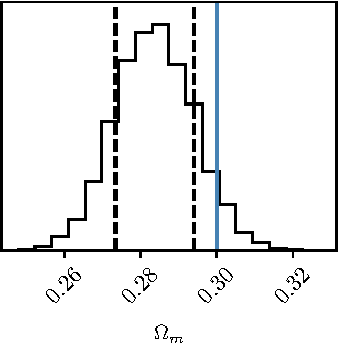
\includegraphics[width=\textwidth]{images/6_MCMC_omega_parameters.pdf}
    \end{minipage}
\caption{\label{fig:MCMC one parameter} Inferred posterior distribution of $\sigma_8$ on the left and $\Omega_m$ on the right. Dotted lines indicate the $1\sigma$ level. Truth values corresponding to the fiducial cosmology are indicated in blue.}
\end{figure}

\subsection{Two parameters}
\subsubsection{Effect of noise}
\begin{table}[h]
\centering
\caption{List of inferred cosmological parameters inferred by the model with a small $32\times32$ grid and for a fixed true GRF realisation. We present the cosmological parameters inferred as we increase the noise level, corresponding to $n_g = 4$, $10$, $30$ and $100 \text{ galaxies}/\text{arcmin}^2$.}\label{tab:inferred cosmological parameters}
\begin{tabular}{lcccc}
    \toprule
    $\sigma_\text{noise}$ & $0.0069$ & $0.0044$ & $0.0025$ & $0.0014$\\
    \midrule
    $S_8$      & $0.716\pm0.043$ & $0.733\pm0.040$ & $0.747\pm0.041$ & $0.752\pm0.042$\\
    $\sigma_8$ & $0.645\pm0.157$ & $0.628\pm0.158$ & $0.632\pm0.166$ & $0.631\pm0.170$\\
    $\Omega_m$ & $0.423\pm0.164$ & $0.469\pm0.175$ & $0.485\pm0.186$ & $0.497\pm0.193$\\
    \bottomrule
\end{tabular}
\end{table}
We perform some tests on low resolution $32\times32$ grids to see the effect that the noise level has on the recovered parameters, see \textit{Tab. }\ref{tab:inferred cosmological parameters}. Here we report the inferred cosmological parameters for one data realisation and different noise levels, corresponding respectively to $n_g = 4$, $10$, $30$ and $100 \text{ galaxies}/\text{arcmin}^2$, see \textit{Eq. }\eqref{eq:noise}. The inferred value of $S_8$ can vary as much as a full $\sigma$ between high and low noise runs. Keeping in mind that $\sigma_8$ and $\Omega_m$ are extremely unreliable due to relative uncertainties of $\sim 25-30\%$ caused by the degeneracy: as a general trend we notice $\Omega_m$ gets bigger when $\sigma_8$ gets smaller with less noise.

\subsubsection{Inferred cosmological parameters}
Running the model for a larger $64\times64$ grid with $n_g=10 \text{ galaxies}/\text{arcmin}^2$, gives much better constraints on the cosmological parameters. We present the values recovered by the posterior distributions, listed as follows in \textit{Tab. }\ref{tab:inferred cosmological parameters (64,64)}. 
\begin{table}[h]
    \centering
    \caption{\label{tab:inferred cosmological parameters (64,64)} Mean and sigma values recovered from the inferred distributions of the cosmological parameters.}
    \begin{tabular}{ccc}
        \toprule
        $S_8$ & $\sigma_8$ & $\Omega_m$\\
        \midrule
        $0.762\pm0.028$ & $0.745\pm0.151$ & $0.353\pm0.143$\\
        \bottomrule
    \end{tabular}
\end{table} 

\textit{Fig. }\ref{fig:MCMC two parameters} shows the inferred posterior distributions and contours for the three cosmological parameters $\sigma_8$, $\Omega_m$ and $S_8$. Looking at the contours, we obtain the well known banana-shaped degeneracy between $\sigma_8$ and $\Omega_m$. The $S_8$ and $\Omega_m$ contour presents sharp cuts for  high and low $\Omega_m$, indicating an issue with the bounds of the uniform priors imposed. Unfortunately the \code{jaxcosmo} package does not allow for the choice of priors to be wider than what shown in \textit{Tab. }\ref{tab:priors}, as the model then starts to have divergent samples.
\begin{figure}[h]
    \centering
    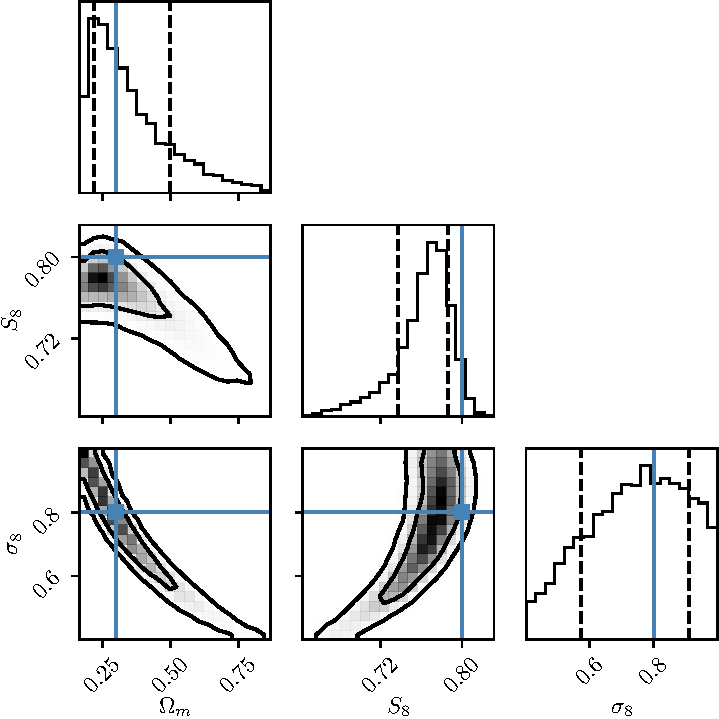
\includegraphics[width=\textwidth]{images/5_MCMC_two_parameters.pdf}
    \caption{\label{fig:MCMC two parameters} Inferred posterior distributions of $S_8$, $\sigma_8$ and $\Omega_m$. For noise level $\sigma_\text{noise}\sim 0.0088$. Contours indicate the $1\sigma$ and $2\sigma$ credible interval respectively. Dotted lines indicate the $1\sigma$ level. Truth values corresponding to the fiducial cosmology are indicated in blue.}
\end{figure}

\subsection{Posterior checks}
Following the two parameter inference model, we perform some posterior checks at the map level \cite{fwdmodel2}. \textit{Fig. }\ref{fig:MCMC summary}
sums up the ability of the model to recover the true map, noiseless and unmasked. Here we present the run with noise level $\sigma_\text{noise}\sim 0.0088$ and a $64\times64$ grid. We show the mean and standard deviation for the sample with highest likelihood out of the $12000$. The mean field $\mu$ is visibly different to the true field in the masked regions and it seems to be of overall lower amplitude. The sample map is comparable to the noisy data; which is to be expected, as the internal noise given to the Gaussian process is the same as the noise level of the data. The standard deviation map $\sigma$ presents an overall amplitude comparable to the noise level $\sim 0.010$, with higher values for the masked regions. Summing up the map values of the residuals divided by standard deviation squared, we obtain a $\chi^2\sim 1297.4$. Compared to the number of free parameters $\nu$ in our inference model, which for a $10\%$ mask and a $64\times64$ grid, is $\nu=3689$. The value of $\chi^2$ therefore seems to be low, indicating that the noise level assumed by the GP is overestimated. This is supported by the fact that the sample map looks just as noisy as the data, according to \textit{Fig. }\ref{fig:residuals vs noise}, its distribution is in fact just as wide as the noise.

\begin{figure}[h]
    \centering
    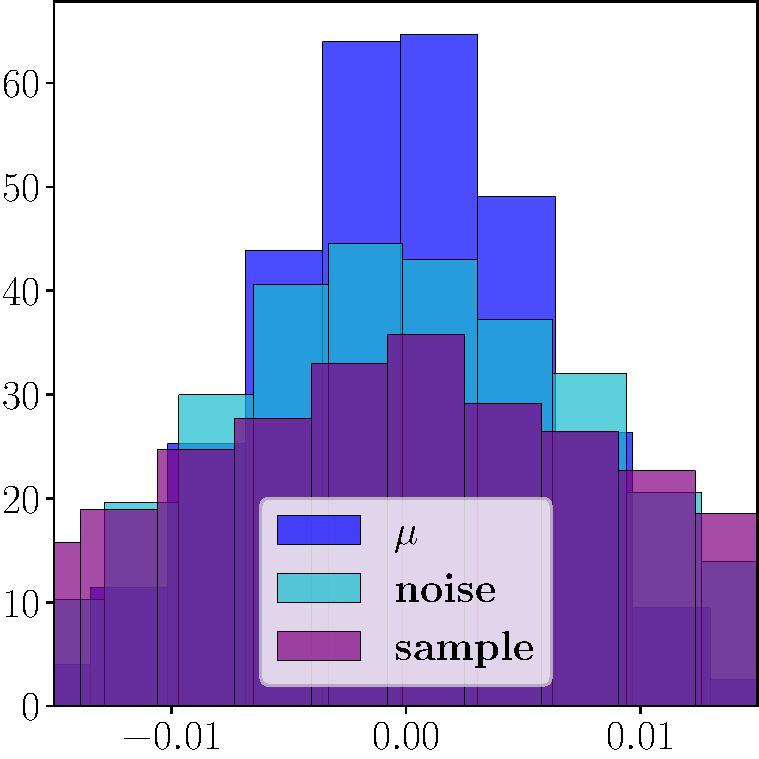
\includegraphics[width=0.5\textwidth]{images/5_residuals_vs_noise.pdf}
    \par \hspace{0.3cm} \textit{Residuals}
    \caption{\label{fig:residuals vs noise} Residual distributions of the mean and sample compared to noise. The mean is less spread, whereas the sample is wider.}
\end{figure}

\begin{figure}[h]
    \centering
    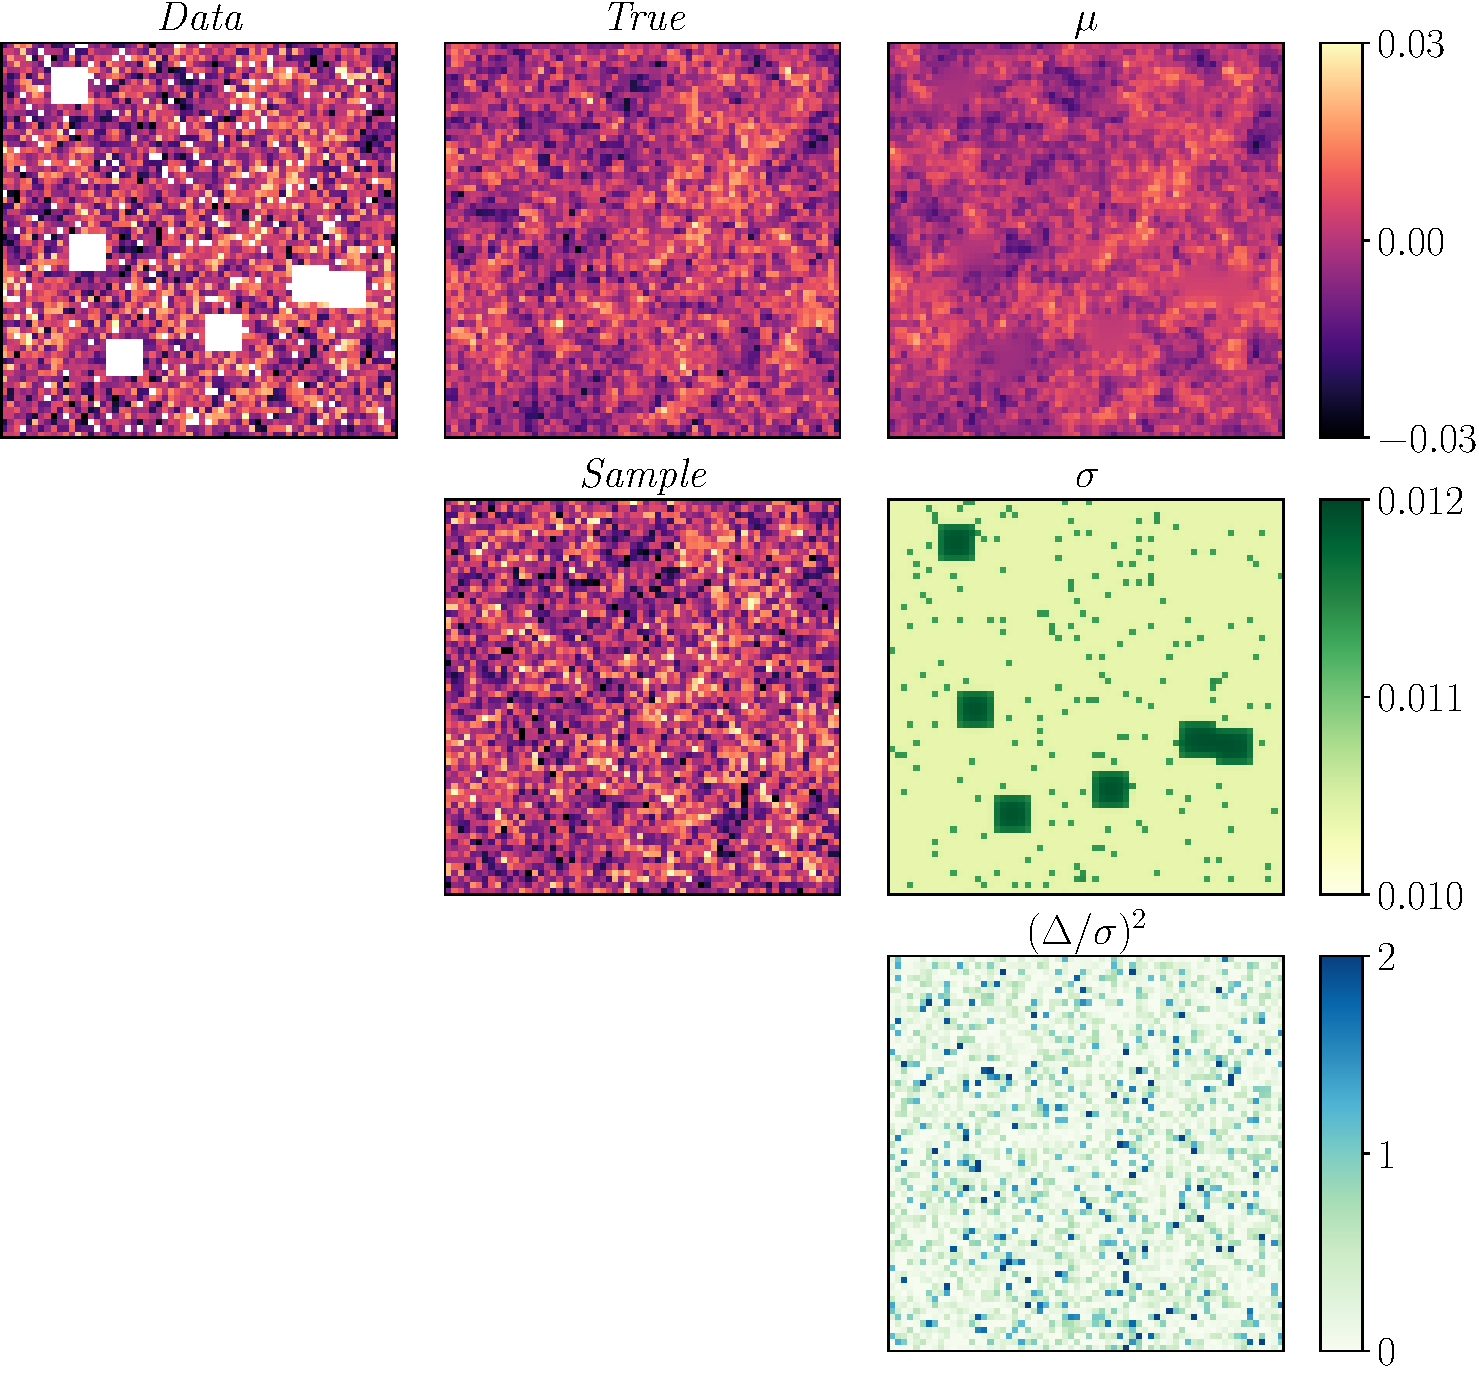
\includegraphics[width=\textwidth]{images/5_summary.pdf}
    \caption{\label{fig:MCMC summary} Summary of the two parameter inference at the map level. The left column shows the masked and noisy GRF realisation used, which is our data. The middle column shows the true GRF and a sample from the conditioned GP. The right column shows maps of the mean, standard deviation and residuals over standard deviation squared resulting from the numpyro model sample with highest likelihood. Regions of higher uncertainty correspond to the masked regions.}
\end{figure}
%%%%%%%%%%%%%%%%%%%%%%%%%%%%%%%%%
%%%%%%%%%%%% CHAPTER %%%%%%%%%%%%
%%%%%%%%%%%%%%%%%%%%%%%%%%%%%%%%%
\chapter{Conclusion}
We have hereby introduced the tool of Gaussian processes to the landscape of map inference of cosmological fields, in particular weak lensing convergence. We considered how the 2-point statistics of cosmological fields changes when we are dealing with bounded and discrete maps in \textit{Sec. }\ref{sec:weak lensing}. We discussed the realisation of Gaussian and lognormal fields in \textit{Sec. }\ref{sec:field generation}, and showed their ability to recover the 2-point statistics that they encode, in \textit{Sec. }\ref{sec:gaussian and lognormal fields}. We have included masking and noise to the data to simulate realistic maps in \textit{Sec. }\ref{sec:data simulation}. We have shown that it is possible to apply physical knowledge about the 2-point correlation function of a cosmological field in order to set up a Gaussian process able to produce a Gaussian realisation of such a field. We considered different set ups for the Gaussian process kernel in \textit{Sec. }\ref{sec:gaussian process kernel} and showed how they fare against one another in \textit{Sec. }\ref{sec:gaussian process priors}, ultimately proving empirically that the half-range FFT model is the best. In \textit{Sec. }\ref{sec:gaussian process map reconstruction} we present an application of Gaussian processes to a noiseless masked convergence map, in order to showcase its ability to reconstruct a heavily masked map. Finally we present our results for the cosmological parameters inference with GPs, conditioning on noisy and masked data. When running the inference model on one cosmological parameter we recover both parameters within two sigmas, $\sigma_8 = 0.776\pm0.015$ and $\Omega_m = 0.284\pm0.010$. For the two parameter inference we observe the well known banana-shaped degeneracy between $\sigma_8$ and $\Omega_m$, as well as recovering $0.762\pm0.028$ within two sigmas.

In future studies GPs could be tested on maps with larger grids. In order to achieve a resolution of $\sim 3$ arcmin with a map of size $(10^\circ,10^\circ)$, a $200\times200$ grid is needed. Too big for a GP. The bottleneck is given by the inversion of the kernel matrix, see \eqref{eq:conditioning}. Approximations of this operation could enable the use of GPs on larger grids. This can lead to the possibility of applying this method on current weak lensing catalogues and perhaps even full sky catalogues. Another pathway to explore are lognormal fields, as they do a much better job at simulating data than GRFs. Due to GPs being Gaussian, their associated likelihood is not suitable to treat lognormal fields. A modified likelihood could therefore unlock a correct application of GPs to lognormal fields.

\section*{Acknowledgments}
This project wouldn't have been possible without the author of the idea, Dr. Tilman Tröster. You guided me through my first real research experience and I am grateful. Thank you Veronika Oehl for always being there and for the very helpful discussions. I also express my gratitude to the Cosmology group at ETH, led by Prof. Alexandre Réfrégier. Hearing about my every progress every Monday morning for six months, couldn't have been easy, thank you. It has been an incredible experience, long and grinding, which I embarked upon with my friends and colleagues Tommaso and Pietro. Thank you for making these past few months memorable. Thanks to Guido van Rossum for giving us \code{Python}. Thank you Mia, for your unconditional support, \textit{you} keep me grounded. Non sarei qua senza di te mamma, grazie.

\bigskip

\noindent
\hfill \llap{\textit{Thank you, reader.}}

\backmatter

\printbibliography %Prints bibliography

\newpage

\begin{tikzpicture}[remember picture,overlay,inner sep=0pt,outer sep=0pt]
\node at (current page.center) {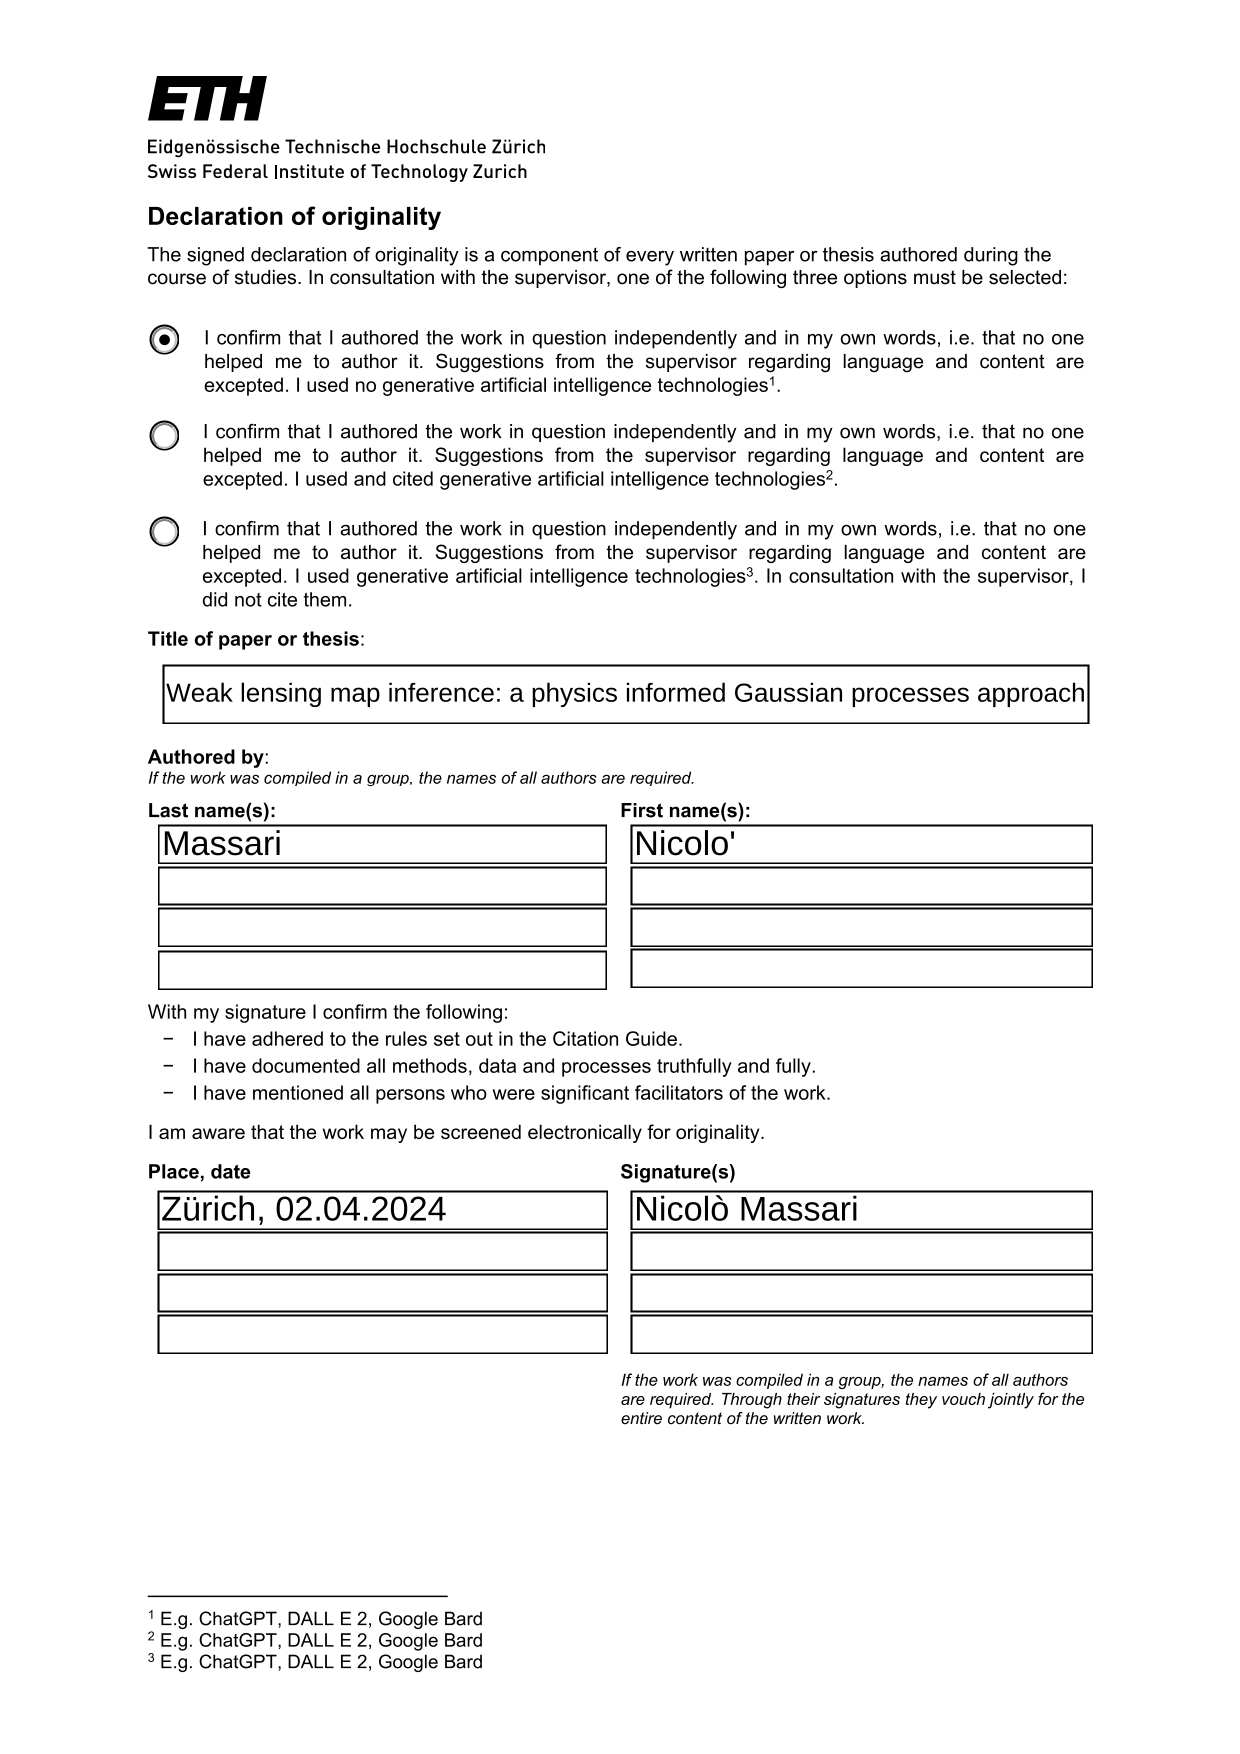
\includegraphics[width=\paperwidth,height=\paperheight]{setup/declaration-originality.pdf}};
\end{tikzpicture}

\clearpage


\end{document}
